\documentclass[aspectratio=169]{beamer}
\usetheme{Madrid}
\usecolortheme{seahorse}
\usepackage{amsmath}
\usepackage{amssymb}
\usepackage{tikz}
\usepackage{algorithm}
\usepackage{algpseudocode}
\usepackage{xcolor}
\usepackage{tcolorbox}
\usepackage{pgfplots}     % This automatically loads the 'tikz' package
\pgfplotsset{compat=1.16} % Good practice for pgfplots
\usetikzlibrary{shapes.geometric, arrows.meta, positioning, calc, patterns}
\usepackage{pifont}           % Provides the dingbat symbols like \ding{55}
\usepackage{newunicodechar}   % Allows you to define Unicode characters
\newunicodechar{✓}{\checkmark}
\newunicodechar{✗}{\ding{55}}

% Custom colors
\definecolor{highDcolor}{RGB}{46, 134, 171}
\definecolor{lowDcolor}{RGB}{162, 59, 114}
\definecolor{gradcolor}{RGB}{255, 127, 14}
\definecolor{gray30}{gray}{0.3}
\definecolor{gray50}{gray}{0.5}
\definecolor{gray70}{gray}{0.7}

% Custom commands
\newcommand{\conceptbox}[2]{\colorbox{#1!20}{\textcolor{#1}{\textbf{#2}}}}
\newcommand{\warning}[1]{\conceptbox{red}{Warning: #1}}
\newcommand{\insight}[1]{\conceptbox{blue}{Insight: #1}}
\newcommand{\ethics}[1]{\conceptbox{purple}{Ethics: #1}}

\title{t-Stochastic Neighbor Embedding}
\author{Prof.Asc. Endri Raco}
\institute{Polytechnic University of Tirane}
\date{October 2025}

\begin{document}


% SLIDE 1: TITLE SLIDE
\begin{frame}
\frametitle{\centering \Large t-SNE: Seeing the Invisible Structure}
\begin{center}
\vspace{0.5cm}
{\large Advanced Multivariate Analysis}\\[0.5cm]
{\normalsize Associate Professor Endri Raco}\\
{\small Polytechnic University of Catalonia}\\[1cm]

\begin{tikzpicture}
% High-dimensional cloud (left)
\begin{scope}[shift={(-3,0)}]
\foreach \i in {1,...,50} {
    \pgfmathsetmacro{\rx}{rand*2-1}
    \pgfmathsetmacro{\ry}{rand*2-1}
    \fill[blue!20, opacity=0.5] (\rx,\ry) circle (0.05);
}
\node[below] at (0,-1.5) {\small Chaos};
\end{scope}

% Arrow
\draw[->, ultra thick, blue!60] (-1,0) -- (1,0);
\node[above] at (0,0) {t-SNE};

% 2D clusters (right)
\begin{scope}[shift={(3,0)}]
\foreach \i in {1,...,10} {
    \pgfmathsetmacro{\rx}{rand*0.3}
    \pgfmathsetmacro{\ry}{rand*0.3+0.7}
    \fill[red!80] (\rx,\ry) circle (0.05);
}
\foreach \i in {1,...,10} {
    \pgfmathsetmacro{\rx}{rand*0.3+0.7}
    \pgfmathsetmacro{\ry}{rand*0.3-0.2}
    \fill[blue!80] (\rx,\ry) circle (0.05);
}
\node[below] at (0,-1.5) {\small Clarity};
\end{scope}
\end{tikzpicture}

\vspace{0.5cm}
{\small \textit{"Finding patterns where none are visible"}}
\end{center}

\note{
[2 min] Welcome! Energy and enthusiasm. Today we master THE tool for high-D visualization.
}
\end{frame}

% SLIDE 2: PERSONAL INTRODUCTION
\begin{frame}
\frametitle{Our Journey Together}
\begin{columns}
\column{0.5\textwidth}
\textbf{This Session:}
\begin{itemize}
\item Exchange of ideas
\item Build intuition first
\item Then mathematics
\item Your questions welcome
\end{itemize}

\column{0.5\textwidth}
\textbf{You'll Master:}
\begin{itemize}
\item \textcolor{blue}{Why} t-SNE works
\item \textcolor{orange}{When} to use it
\item \textcolor{green}{How} to implement
\item \textcolor{red}{Pitfalls} to avoid
\end{itemize}
\end{columns}

\vspace{0.5cm}
\centering
\textit{"By the end, you'll see data differently"}

\note{
[1 min] Set expectations. Interactive, not passive.
}
\end{frame}

% SLIDE 3: THE DATA CHALLENGE
\begin{frame}
\frametitle{The Data Visualization Challenge}
\begin{columns}
\column{0.45\textwidth}
\textbf{Single-cell RNA}\\
\textbf{20,000 dimensions!}\\[0.3cm]
\tiny
\begin{tabular}{|c|c|c|c|}
\hline
Cell & Gene1 & Gene2 & ...\\
\hline
1 & 0.23 & 1.45 & ...\\
2 & 0.67 & 0.89 & ...\\
3 & 1.23 & 0.02 & ...\\
... & ... & ... & ...\\
\hline
\end{tabular}

\vspace{0.3cm}
\normalsize
\textcolor{red}{How find cell types?}

\column{0.45\textwidth}
\textbf{After t-SNE:}\\[0.3cm]
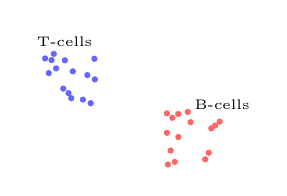
\begin{tikzpicture}[scale=0.8]
% T-cells cluster
\foreach \i in {1,...,15} {
    \pgfmathsetmacro{\rx}{rand*0.5}
    \pgfmathsetmacro{\ry}{rand*0.5+2}
    \fill[blue!60] (\rx,\ry) circle (0.05);
}
% B-cells cluster
\foreach \i in {1,...,15} {
    \pgfmathsetmacro{\rx}{rand*0.5+2}
    \pgfmathsetmacro{\ry}{rand*0.5+1}
    \fill[red!60] (\rx,\ry) circle (0.05);
}
\node at (0,2.5) {\tiny T-cells};
\node at (2.5,1.5) {\tiny B-cells};
\end{tikzpicture}

\vspace{0.3cm}
\textcolor{green}{Cell types visible!}
\end{columns}

\note{
[2 min] Hook with real impact. Pause for effect after showing transformation.
}
\end{frame}

% SLIDE 4: CURSE OF DIMENSIONALITY - INTUITION
\begin{frame}
\frametitle{The Curse: A Thought Experiment}

\centering
\textbf{Finding Your Friend at a Concert}\\[0.5cm]

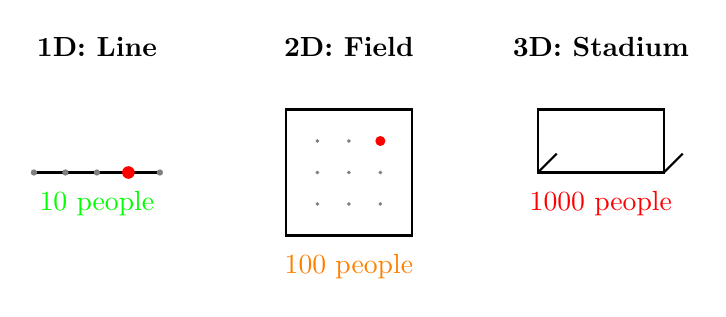
\begin{tikzpicture}[scale=0.8]
% 1D
\node at (-4,2) {\textbf{1D: Line}};
\draw[thick] (-5,0) -- (-3,0);
\foreach \x in {-5,-4.5,...,-3}
    \fill[gray] (\x,0) circle (0.05);
\fill[red] (-3.5,0) circle (0.1);
\node at (-4,-0.5) {\textcolor{green}{10 people}};

% 2D
\node at (0,2) {\textbf{2D: Field}};
\draw[thick] (-1,-1) rectangle (1,1);
\foreach \x in {-0.5,0,0.5}
    \foreach \y in {-0.5,0,0.5}
        \fill[gray] (\x,\y) circle (0.03);
\fill[red] (0.5,0.5) circle (0.08);
\node at (0,-1.5) {\textcolor{orange}{100 people}};

% 3D hint
\node at (4,2) {\textbf{3D: Stadium}};
\draw[thick] (3,0) -- (5,0) -- (5,1) -- (3,1) -- cycle;
\draw[thick] (3,0) -- (3.3,0.3);
\draw[thick] (5,0) -- (5.3,0.3);
\node at (4,-0.5) {\textcolor{red}{1000 people}};
\end{tikzpicture}

\vspace{0.5cm}
\textbf{In 20,000 dimensions?}\\
Your friend is \textit{everywhere and nowhere}

\note{
[2 min] Interactive - ask students to imagine. Build intuition first!
}
\end{frame}

% SLIDE 5: CURSE - MATHEMATICAL
\begin{frame}
\frametitle{The Curse: Mathematics}

\begin{columns}
\column{0.5\textwidth}
\textbf{Volume in n-dim sphere:}
$$V_n(r) = \frac{\pi^{n/2}}{\Gamma(n/2 + 1)} r^n$$

\vspace{0.3cm}
\textbf{Shell vs Core:}
$$\frac{V_{shell}}{V_{total}} = 1 - (0.99)^n$$

\column{0.5\textwidth}
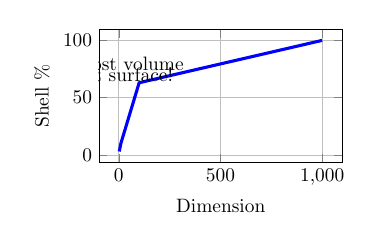
\begin{tikzpicture}[scale=0.7]
\begin{axis}[
    xlabel={Dimension},
    ylabel={Shell \%},
    grid=major,
    width=6cm,
    height=4cm
]
\addplot[blue, ultra thick] coordinates {
    (2,3) (10,10) (100,63) (1000,99.99)
};
\node at (axis cs: 50,80) {Most volume};
\node at (axis cs: 50,70) {at surface!};
\end{axis}
\end{tikzpicture}
\end{columns}

\vspace{0.5cm}
\centering
\textbf{Key Insight:} All points become equally distant!

\note{
[2 min] Mathematical proof. Emphasize counterintuitive nature.
}
\end{frame}

% SLIDE 6: DISTANCE DISTRIBUTIONS
\begin{frame}
\frametitle{Distance Collapse}

\begin{center}
\textbf{Random points in hypercube}\\[0.3cm]

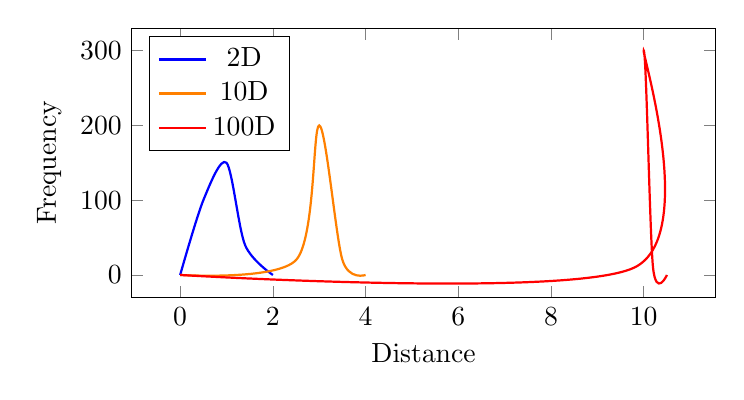
\begin{tikzpicture}
\begin{axis}[
    xlabel={Distance},
    ylabel={Frequency},
    width=9cm,
    height=5cm,
    legend pos=north west
]
% 2D - wide distribution
\addplot[blue, thick, smooth] coordinates {
    (0,0) (0.5,100) (1,150) (1.4,40) (2,0)
};
\addlegendentry{2D}

% 10D - narrower
\addplot[orange, thick, smooth] coordinates {
    (0,0) (2.5,20) (3.0,200) (3.5,20) (4,0)
};
\addlegendentry{10D}

% 100D - very narrow
\addplot[red, thick, smooth] coordinates {
    (0,0) (9.8,10) (10,300) (10.2,10) (10.5,0)
};
\addlegendentry{100D}
\end{axis}
\end{tikzpicture}
\end{center}

\textbf{Problem:} No meaningful neighborhoods!

\note{
[1.5 min] Visual proof. Ask: "How find structure when all equally far?"
}
\end{frame}

% SLIDE 7: PCA FAILS
\begin{frame}
\frametitle{Why PCA Fails}

\begin{center}
\textbf{The Swiss Roll Problem}\\[0.5cm]

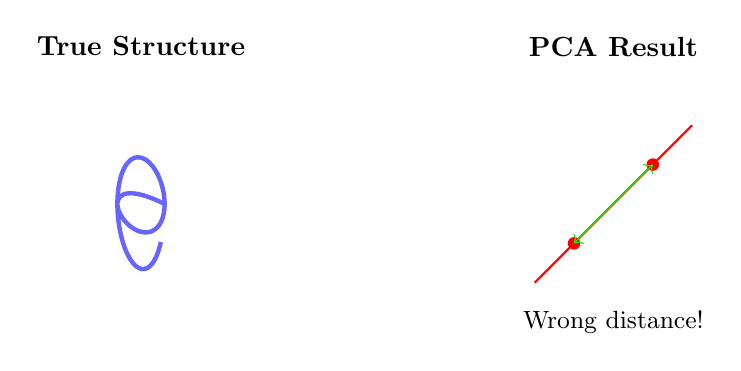
\begin{tikzpicture}[scale=1]
% Swiss roll
\node at (-3,2) {\textbf{True Structure}};
\draw[ultra thick, blue!60] plot[domain=0:12, samples=50, smooth]
    ({-3+0.3*cos(\x r)}, {0.3*\x*sin(\x r)/4});

% PCA projection
\node at (3,2) {\textbf{PCA Result}};
\draw[thick, red] (2,-1) -- (4,1);
\fill[red] (2.5,-0.5) circle (0.08);
\fill[red] (3.5,0.5) circle (0.08);
\draw[<->, green] (2.5,-0.5) -- (3.5,0.5);
\node at (3,-1.5) {\small Wrong distance!};
\end{tikzpicture}
\end{center}

PCA assumes linear subspace - misses manifold structure

\note{
[2 min] Classic example. PCA destroys local neighborhoods.
}
\end{frame}

% SLIDE 8: MDS CROWDING
\begin{frame}
\frametitle{MDS: The Crowding Problem}

\begin{columns}
\column{0.5\textwidth}
\centering
\textbf{Original: 3D}\\
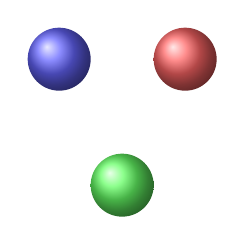
\begin{tikzpicture}[scale=0.8]
\shade[ball color=blue!60] (0,2) circle (0.5);
\shade[ball color=red!60] (2,2) circle (0.5);
\shade[ball color=green!60] (1,0) circle (0.5);
\end{tikzpicture}\\
3 separate clusters

\column{0.5\textwidth}
\centering
\textbf{MDS in 2D}\\
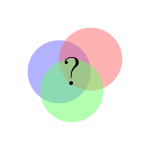
\begin{tikzpicture}[scale=0.8]
\fill[blue!60, opacity=0.5] (0.5,1) circle (0.5);
\fill[red!60, opacity=0.5] (1,1.2) circle (0.5);
\fill[green!60, opacity=0.5] (0.7,0.7) circle (0.5);
\node at (0.7,1) {\Large ?};
\end{tikzpicture}\\
\textcolor{red}{Overlap!}
\end{columns}

\vspace{0.5cm}
\centering
Not enough "room" in 2D for all distances

\note{
[1.5 min] Why equal weight to all distances fails.
}
\end{frame}

% SLIDE 9: MANIFOLD HYPOTHESIS
\begin{frame}
\frametitle{The Manifold Hypothesis}

\begin{center}
\textbf{High-D data lies on low-D manifolds}\\[0.5cm]

\begin{columns}
\column{0.33\textwidth}
\centering
\textbf{Earth}\\
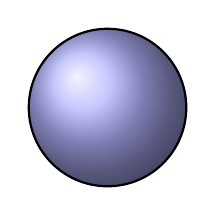
\begin{tikzpicture}[scale=0.5]
\shade[ball color=blue!30] (0,0) circle (2);
\draw[thick] (0,0) circle (2);
\end{tikzpicture}\\
3D sphere\\
$\downarrow$\\
2D surface

\column{0.33\textwidth}
\centering
\textbf{Faces}\\

\begin{tikzpicture}[scale=0.6]
\draw[thick] (0,0) circle (1);
\fill (0.3,0.3) circle (0.1);
\fill (-0.3,0.3) circle (0.1);
\draw (-0.3,-0.3) arc (180:360:0.3);
\end{tikzpicture}\\
10K pixels\\
$\downarrow$\\
~50 dimensions

\column{0.33\textwidth}
\centering
\textbf{Words}\\
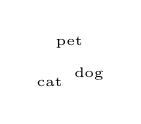
\begin{tikzpicture}[scale=0.5]
\node at (0,0) {\tiny cat};
\node at (1,0.2) {\tiny dog};
\node at (0.5,1) {\tiny pet};
\end{tikzpicture}\\
Vocabulary\\
$\downarrow$\\
~300D semantic
\end{columns}
\end{center}

\textbf{Key:} True complexity $\ll$ apparent dimensions

\note{
[2 min] Connect to everyday examples. Make abstract tangible.
}
\end{frame}

% SLIDE 10: t-SNE PROMISE
\begin{frame}
\frametitle{t-SNE's Revolutionary Promise}

\begin{center}
\textbf{MNIST Digits: 784D $\rightarrow$ 2D}\\[0.3cm]

\begin{columns}
\column{0.5\textwidth}
\centering
\textbf{PCA}\\
\begin{tikzpicture}[scale=0.6]
\foreach \i in {1,...,30} {
    \pgfmathsetmacro{\rx}{rand*4}
    \pgfmathsetmacro{\ry}{rand*4}
    \fill[blue!40, opacity=0.5] (\rx,\ry) circle (0.08);
}
\node at (2,-0.5) {\small Mixed};
\end{tikzpicture}

\column{0.5\textwidth}
\centering
\textbf{t-SNE}\\
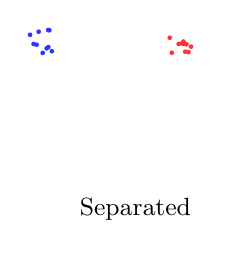
\begin{tikzpicture}[scale=0.6]
\foreach \i in {1,...,10} {
    \pgfmathsetmacro{\rx}{rand*0.3}
    \pgfmathsetmacro{\ry}{rand*0.3+3}
    \fill[blue!80] (\rx,\ry) circle (0.05);
}
\foreach \i in {1,...,10} {
    \pgfmathsetmacro{\rx}{rand*0.3+3}
    \pgfmathsetmacro{\ry}{rand*0.3+3}
    \fill[red!80] (\rx,\ry) circle (0.05);
}
\node at (2,-0.5) {\small Separated};
\end{tikzpicture}
\end{columns}
\end{center}

\vspace{0.5cm}
\centering
\Large{\textcolor{blue}{Key: Preserve neighborhoods, not distances}}

\note{
[2 min] Dramatic reveal. Show actual impact.
}
\end{frame}

% SLIDE 11: FUNDAMENTAL INSIGHT
\begin{frame}
\frametitle{The Fundamental Insight}

\begin{center}
\textbf{Local vs Global}\\[0.5cm]

\begin{tikzpicture}[scale=1.2]
% High-D
\node at (-3,2) {\textbf{High-D}};
\fill[blue] (-3,0) circle (0.1);
\foreach \a in {0,45,...,315}
    \fill[green] ({-3+0.5*cos(\a)},{0.5*sin(\a)}) circle (0.05);
\foreach \a in {0,30,...,330}
    \fill[gray!30] ({-3+1.5*cos(\a)},{1.5*sin(\a)}) circle (0.03);

\draw[->, ultra thick] (-1,0) -- (1,0);
\node[above] at (0,0) {t-SNE};

% Low-D
\node at (3,2) {\textbf{2D}};
\fill[blue] (3,0) circle (0.1);
\foreach \a in {0,45,...,315}
    \fill[green] ({3+0.5*cos(\a)},{0.5*sin(\a)}) circle (0.05);
% Gray scattered
\fill[gray!30] (4.5,1) circle (0.03);
\fill[gray!30] (1.5,0.5) circle (0.03);
\end{tikzpicture}
\end{center}

\begin{itemize}
\item \textcolor{green}{\checkmark Keep nearby points together}
\item \textcolor{gray}{$\circ$ Let distant points reorganize}
\end{itemize}

\note{
[1.5 min] Core principle. Friends vs acquaintances analogy.
}
\end{frame}

% SLIDE 12: ROADMAP
\begin{frame}
\frametitle{Our Learning Journey}

\begin{center}
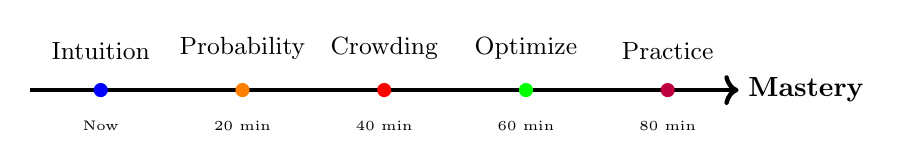
\begin{tikzpicture}[scale=0.9]
\draw[ultra thick, ->] (0,0) -- (10,0);
\node[right] at (10,0) {\textbf{Mastery}};

% Milestones
\fill[blue] (1,0) circle (0.1);
\node[above] at (1,0.3) {\small Intuition};
\node[below] at (1,-0.3) {\tiny Now};

\fill[orange] (3,0) circle (0.1);
\node[above] at (3,0.3) {\small Probability};
\node[below] at (3,-0.3) {\tiny 20 min};

\fill[red] (5,0) circle (0.1);
\node[above] at (5,0.3) {\small Crowding};
\node[below] at (5,-0.3) {\tiny 40 min};

\fill[green] (7,0) circle (0.1);
\node[above] at (7,0.3) {\small Optimize};
\node[below] at (7,-0.3) {\tiny 60 min};

\fill[purple] (9,0) circle (0.1);
\node[above] at (9,0.3) {\small Practice};
\node[below] at (9,-0.3) {\tiny 80 min};
\end{tikzpicture}
\end{center}

\vspace{0.5cm}
\centering
Questions welcome at each checkpoint!

\note{
[1 min] Set expectations. Structured progression.
}
\end{frame}

% SLIDE 13: PART 2 TITLE
\begin{frame}
\frametitle{Part 2: From Distances to Probabilities}

\begin{center}
\LARGE{\textbf{The Core Innovation}}\\[1cm]

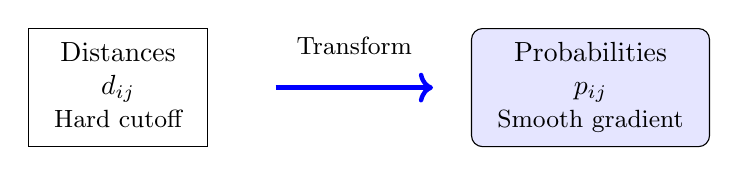
\begin{tikzpicture}[scale=1]
\node[draw, rectangle] at (-3,0) {
    \begin{tabular}{c}
    Distances\\
    $d_{ij}$\\
    \small Hard cutoff
    \end{tabular}
};

\draw[->, ultra thick, blue] (-1,0) -- (1,0);
\node[above] at (0,0.3) {\small Transform};

\node[draw, rounded corners, fill=blue!10] at (3,0) {
    \begin{tabular}{c}
    Probabilities\\
    $p_{ij}$\\
    \small Smooth gradient
    \end{tabular}
};
\end{tikzpicture}
\end{center}

\note{
[2 min] Major transition. Explain why probabilities are genius.
}
\end{frame}

% SLIDE 14: FRIENDS ANALOGY
\begin{frame}
\frametitle{The "Friends" Analogy}

\begin{columns}
\column{0.5\textwidth}
\textbf{Your Social Network}\\[0.3cm]
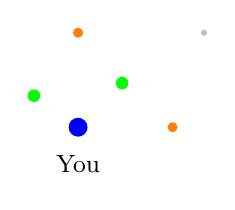
\begin{tikzpicture}[scale=0.8]
\fill[blue] (0,0) circle (0.15);
\node[below] at (0,-0.3) {\small You};
% Close friends
\fill[green] (0.7,0.7) circle (0.1);
\fill[green] (-0.7,0.5) circle (0.1);
% Acquaintances
\fill[orange] (1.5,0) circle (0.08);
\fill[orange] (0,1.5) circle (0.08);
% Strangers
\fill[gray!50] (2,1.5) circle (0.05);
\end{tikzpicture}

\column{0.5\textwidth}
\textbf{Picking Probability}\\[0.3cm]
\begin{tabular}{lr}
Best friend: & 40\%\\
Close friends: & 30\%\\
Acquaintances: & 25\%\\
Strangers: & 5\%\\
\end{tabular}

\vspace{0.3cm}
Closer = Higher probability
\end{columns}

\vspace{0.5cm}
\centering
t-SNE does this for \textbf{every} point!

\note{
[2 min] Relatable analogy. Everyone understands social circles.
}
\end{frame}

% SLIDE 15: GAUSSIAN KERNEL
\begin{frame}
\frametitle{The Gaussian Kernel}

\begin{center}
$$p_{j|i} = \frac{\exp(-d_{ij}^2 / 2\sigma_i^2)}{\sum_{k \neq i} \exp(-d_{ik}^2 / 2\sigma_i^2)}$$
\end{center}

\begin{columns}
\column{0.5\textwidth}
\centering
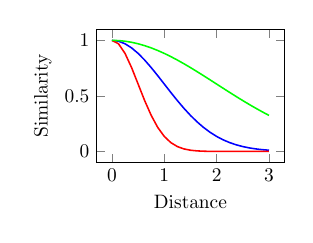
\begin{tikzpicture}[scale=0.7]
\begin{axis}[
    xlabel={Distance},
    ylabel={Similarity},
    width=5cm,
    height=4cm
]
\addplot[blue, thick, domain=0:3] {exp(-x^2/2)};
\addplot[red, thick, domain=0:3] {exp(-x^2/0.5)};
\addplot[green, thick, domain=0:3] {exp(-x^2/8)};
\end{axis}
\end{tikzpicture}

\column{0.5\textwidth}
\textbf{Effect of $\sigma_i$:}
\begin{itemize}
\item \textcolor{red}{Small}: Very local
\item \textcolor{blue}{Medium}: Balanced
\item \textcolor{green}{Large}: Global view
\end{itemize}

Each point gets its own $\sigma_i$!
\end{columns}

\note{
[2 min] Show adaptive bandwidth. Key innovation.
}
\end{frame}

% SLIDE 16: STEP BY STEP
\begin{frame}
\frametitle{Building the Probabilities}

\begin{enumerate}
\item \textbf{Compute distances}
$$d_{ij} = ||x_i - x_j||$$

\item \textbf{Apply Gaussian}
$$\tilde{p}_{j|i} = \exp(-d_{ij}^2 / 2\sigma_i^2)$$

\item \textbf{Normalize}
$$p_{j|i} = \frac{\tilde{p}_{j|i}}{\sum_{k \neq i} \tilde{p}_{k|i}}$$

\item \textbf{Interpretation}
\colorbox{yellow!20}{Probability that $i$ picks $j$ as neighbor}
\end{enumerate}

\note{
[1.5 min] Build systematically. Check understanding.
}
\end{frame}

% SLIDE 17: WORKED EXAMPLE
\begin{frame}
\frametitle{Example: 5 Points}

\begin{columns}
\column{0.4\textwidth}
\centering
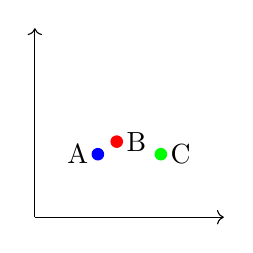
\begin{tikzpicture}[scale=0.8]
\draw[->] (0,0) -- (3,0);
\draw[->] (0,0) -- (0,3);
\fill[blue] (1,1) circle (0.1);
\node[left] at (1,1) {A};
\fill[red] (1.3,1.2) circle (0.1);
\node[right] at (1.3,1.2) {B};
\fill[green] (2,1) circle (0.1);
\node[right] at (2,1) {C};
\end{tikzpicture}

\column{0.6\textwidth}
\textbf{From A's perspective:}\\
\small
\begin{tabular}{l|c|c}
Point & Distance & $p_{j|A}$\\
\hline
B & 0.36 & \textcolor{green}{51\%}\\
C & 1.00 & 9\%\\
Others & >1.5 & <1\%\\
\end{tabular}

\vspace{0.3cm}
B is A's primary neighbor
\end{columns}

\note{
[2 min] Concrete numbers make it real.
}
\end{frame}

% SLIDE 18: PERPLEXITY CONCEPT
\begin{frame}
\frametitle{Perplexity: The Key Parameter}

\begin{center}
\Large{\textbf{Perplexity = "How many neighbors?"}}\\[0.5cm]

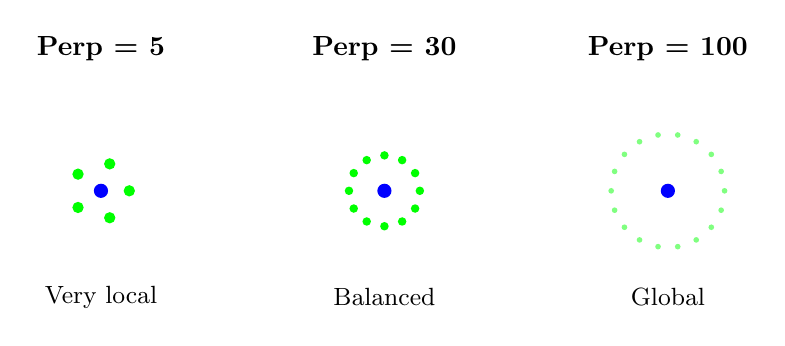
\begin{tikzpicture}[scale=0.9]
% Low
\node at (-4,2) {\textbf{Perp = 5}};
\fill[blue] (-4,0) circle (0.1);
\foreach \a in {0,72,...,288}
    \fill[green] ({-4+0.4*cos(\a)},{0.4*sin(\a)}) circle (0.08);
\node at (-4,-1.5) {\small Very local};

% Medium
\node at (0,2) {\textbf{Perp = 30}};
\fill[blue] (0,0) circle (0.1);
\foreach \a in {0,30,...,330}
    \fill[green] ({0.5*cos(\a)},{0.5*sin(\a)}) circle (0.06);
\node at (0,-1.5) {\small Balanced};

% High
\node at (4,2) {\textbf{Perp = 100}};
\fill[blue] (4,0) circle (0.1);
\foreach \a in {0,20,...,340}
    \fill[green!50] ({4+0.8*cos(\a)},{0.8*sin(\a)}) circle (0.04);
\node at (4,-1.5) {\small Global};
\end{tikzpicture}
\end{center}

\note{
[2 min] Critical parameter. Show visual impact.
}
\end{frame}

% SLIDE 19: PERPLEXITY EFFECTS
\begin{frame}
\frametitle{Perplexity in Action}

\begin{center}
\textbf{Same data, different perplexity}\\[0.3cm]

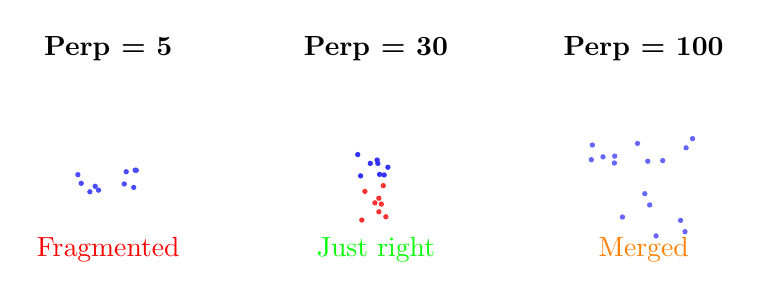
\begin{tikzpicture}[scale=0.85]
% Perp 5
\begin{scope}[shift={(-4,0)}]
\node at (0,2) {\textbf{Perp = 5}};
\foreach \i in {1,...,5} {
    \pgfmathsetmacro{\rx}{rand*0.2-0.3}
    \pgfmathsetmacro{\ry}{rand*0.2}
    \fill[blue!70] (\rx,\ry) circle (0.04);
}
\foreach \i in {1,...,5} {
    \pgfmathsetmacro{\rx}{rand*0.2+0.3}
    \pgfmathsetmacro{\ry}{rand*0.2}
    \fill[blue!70] (\rx,\ry) circle (0.04);
}
\node at (0,-1) {\textcolor{red}{Fragmented}};
\end{scope}

% Perp 30
\begin{scope}[shift={(0,0)}]
\node at (0,2) {\textbf{Perp = 30}};
\foreach \i in {1,...,8} {
    \pgfmathsetmacro{\rx}{rand*0.3}
    \pgfmathsetmacro{\ry}{rand*0.3+0.3}
    \fill[blue!80] (\rx,\ry) circle (0.04);
}
\foreach \i in {1,...,8} {
    \pgfmathsetmacro{\rx}{rand*0.3}
    \pgfmathsetmacro{\ry}{rand*0.3-0.3}
    \fill[red!80] (\rx,\ry) circle (0.04);
}
\node at (0,-1) {\textcolor{green}{Just right}};
\end{scope}

% Perp 100
\begin{scope}[shift={(4,0)}]
\node at (0,2) {\textbf{Perp = 100}};
\foreach \i in {1,...,16} {
    \pgfmathsetmacro{\rx}{rand*0.8}
    \pgfmathsetmacro{\ry}{rand*0.8}
    \fill[blue!60] (\rx,\ry) circle (0.04);
}
\node at (0,-1) {\textcolor{orange}{Merged}};
\end{scope}
\end{tikzpicture}
\end{center}

\colorbox{yellow!20}{Rule: Perplexity between 5 and 50}

\note{
[1.5 min] Most common user error!
}
\end{frame}

% SLIDE 20: FINDING SIGMA
\begin{frame}
\frametitle{Finding the Right $\sigma_i$}

\begin{center}
\textbf{Binary Search for Each Point}\\[0.5cm]

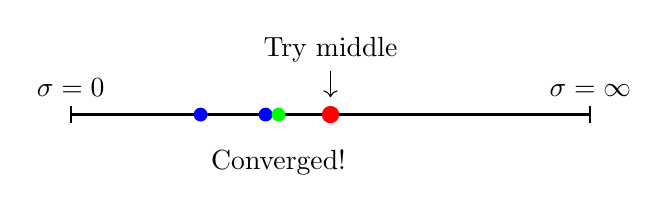
\begin{tikzpicture}[scale=1.1]
\draw[thick] (0,0) -- (6,0);
\draw[thick] (0,-0.1) -- (0,0.1);
\node[above] at (0,0.1) {$\sigma=0$};
\draw[thick] (6,-0.1) -- (6,0.1);
\node[above] at (6,0.1) {$\sigma=\infty$};

% Iterations
\fill[red] (3,0) circle (0.1);
\draw[->] (3,0.5) -- (3,0.2);
\node[above] at (3,0.5) {Try middle};

\fill[blue] (1.5,0) circle (0.08);
\fill[blue] (2.25,0) circle (0.08);
\fill[green] (2.4,0) circle (0.08);
\node[below] at (2.4,-0.3) {Converged!};
\end{tikzpicture}
\end{center}

\begin{itemize}
\item Target: perplexity $\rightarrow$ entropy
\item Adjust $\sigma$ until match
\item Converges in ~10 iterations
\item Do this for ALL $n$ points!
\end{itemize}

\note{
[2 min] Computational detail but important.
}
\end{frame}

% SLIDE 21: MATHEMATICAL PERPLEXITY
\begin{frame}
\frametitle{Perplexity: The Math}

\begin{definition}[Perplexity]
$$\text{Perp}(P_i) = 2^{H(P_i)}$$
where entropy:
$$H(P_i) = -\sum_j p_{j|i} \log_2 p_{j|i}$$
\end{definition}

\textbf{Interpretation:}
\begin{itemize}
\item Effective number of neighbors
\item Perp = 30 $\approx$ 30 equally likely neighbors
\item Controls local vs global focus
\end{itemize}

\textbf{Binary search finds $\sigma_i$ such that:}
$$\text{Perp}(P_i) = \text{user specified perplexity}$$

\note{
[1.5 min] Connect math to intuition.
}
\end{frame}

% SLIDE 22: COMMON PERPLEXITY MISTAKES
\begin{frame}
\frametitle{Perplexity Pitfalls}

\begin{center}
\textbf{Common Mistakes}\\[0.5cm]

\begin{tabular}{l|l|l}
\textbf{Setting} & \textbf{Result} & \textbf{Fix}\\
\hline
Perp = 2 & Islands & Increase to 15+\\
Perp = 200 & Blob & Decrease to 50\\
Perp > n/3 & Unstable & Use 5-50 range\\
\end{tabular}
\end{center}

\vspace{0.5cm}
\textbf{Best Practice:}
\begin{itemize}
\item Try multiple values (15, 30, 50)
\item Look for stable patterns
\item Consider data size: larger n $\rightarrow$ larger perp OK
\end{itemize}

\note{
[1.5 min] Practical guidance critical.
}
\end{frame}

% SLIDE 23: SYMMETRIZATION NEED
\begin{frame}
\frametitle{The Asymmetry Problem}

\begin{center}
\textbf{$p_{j|i} \neq p_{i|j}$}\\[0.5cm]

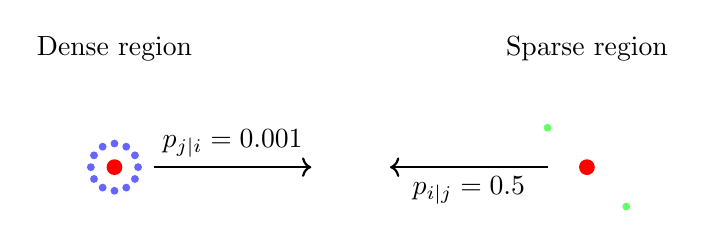
\begin{tikzpicture}[scale=1]
% Dense region
\node at (-3,1.5) {Dense region};
\foreach \a in {0,30,...,330}
    \fill[blue!60] ({-3+0.3*cos(\a)},{0.3*sin(\a)}) circle (0.05);
\fill[red] (-3,0) circle (0.1);

% Sparse region
\node at (3,1.5) {Sparse region};
\fill[green!60] (2.5,0.5) circle (0.05);
\fill[green!60] (3.5,-0.5) circle (0.05);
\fill[red] (3,0) circle (0.1);

% Arrows
\draw[->, thick] (-2.5,0) -- (-0.5,0);
\node[above] at (-1.5,0) {$p_{j|i}=0.001$};
\draw[->, thick] (2.5,0) -- (0.5,0);
\node[below] at (1.5,0) {$p_{i|j}=0.5$};
\end{tikzpicture}
\end{center}

\textcolor{red}{Problem: Outliers pull but aren't pulled!}

\note{
[2 min] Critical issue - motivate symmetrization.
}
\end{frame}

% SLIDE 24: SYMMETRIZATION SOLUTION
\begin{frame}
\frametitle{Symmetrization Solution}

\begin{columns}
\column{0.5\textwidth}
\textbf{Simple Fix:}
$$p_{ij} = \frac{p_{j|i} + p_{i|j}}{2n}$$

\vspace{0.3cm}
\textbf{Properties:}
\begin{itemize}
\item Symmetric
\item Sum to 1
\item Fair to all points
\end{itemize}

\column{0.5\textwidth}
\textbf{Example:}\\
Before:\\
$p_{j|i} = 0.001$\\
$p_{i|j} = 0.500$\\[0.3cm]
After:\\
$p_{ij} = 0.250/n$\\
$p_{ji} = 0.250/n$\\[0.3cm]
\textcolor{green}{Balanced!}
\end{columns}

\note{
[1.5 min] Elegant solution to asymmetry.
}
\end{frame}

% SLIDE 25: NORMALIZATION CHECK
\begin{frame}
\frametitle{Mathematical Check}

\begin{theorem}[Joint Distribution]
With $p_{ij} = \frac{p_{j|i} + p_{i|j}}{2n}$:
$$\sum_{i,j} p_{ij} = 1$$
\end{theorem}

\textbf{Proof:}
\begin{align*}
\sum_{i,j} p_{ij} &= \sum_{i,j} \frac{p_{j|i} + p_{i|j}}{2n}\\
&= \frac{1}{2n} \left[\sum_{i,j} p_{j|i} + \sum_{i,j} p_{i|j}\right]\\
&= \frac{1}{2n} [n + n] = 1 \quad \checkmark
\end{align*}

\note{
[1.5 min] Mathematical rigor - it works!
}
\end{frame}

% SLIDE 26: PART 3 TITLE
\begin{frame}
\frametitle{Part 3: The Crowding Problem}

\begin{center}
\LARGE{\textbf{Why Gaussians Fail}}\\[0.5cm]

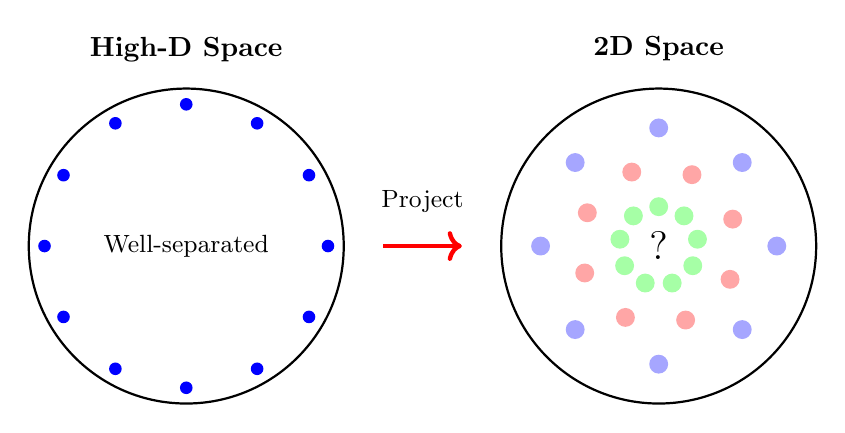
\begin{tikzpicture}[scale=1]
% High-D space (many points well-separated)
\node at (-3,2.5) {\textbf{High-D Space}};
\draw[thick] (-3,0) circle (2);
\foreach \a in {0,30,...,330} {
    \fill[blue] ({-3+1.8*cos(\a)},{1.8*sin(\a)}) circle (0.08);
}
\node at (-3,0) {\small Well-separated};

% Arrow showing projection
\draw[->, ultra thick, red] (-0.5,0) -- (0.5,0);
\node[above] at (0,0.3) {\small Project};

% 2D space (crowded points)
\node at (3,2.5) {\textbf{2D Space}};
\draw[thick] (3,0) circle (2);
% Overlapping points showing crowding
\foreach \a in {0,45,...,315} {
    \fill[blue!50, opacity=0.7] ({3+1.5*cos(\a)},{1.5*sin(\a)}) circle (0.12);
}
\foreach \a in {20,65,...,335} {
    \fill[red!50, opacity=0.7] ({3+1*cos(\a)},{1*sin(\a)}) circle (0.12);
}
\foreach \a in {10,50,...,340} {
    \fill[green!50, opacity=0.7] ({3+0.5*cos(\a)},{0.5*sin(\a)}) circle (0.12);
}
\node at (3,0) {\Large ?};
\end{tikzpicture}

\vspace{0.3cm}
\textcolor{red}{Not enough "room" in 2D!}
\end{center}

\note{
[2 min] Major transition - the core problem.
}
\end{frame}

% SLIDE 27: VOLUME SCALING
\begin{frame}
\frametitle{Volume Scaling Problem}

\begin{columns}
\column{0.5\textwidth}
\textbf{Volume ratio:}
$$\frac{V_n(2r)}{V_n(r)} = 2^n$$

\vspace{0.3cm}
\textbf{Examples:}
\begin{itemize}
\item 2D: $2^2 = 4\times$
\item 10D: $2^{10} = 1024\times$
\item 100D: $2^{100} \approx 10^{30}\times$
\end{itemize}

\column{0.5\textwidth}
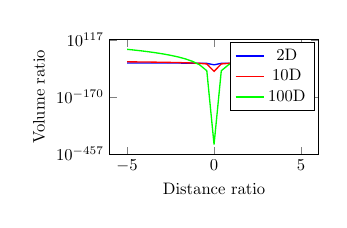
\begin{tikzpicture}[scale=0.6]
\begin{axis}[
    xlabel={Distance ratio},
    ylabel={Volume ratio},
    ymode=log,
    width=6cm,
    height=4cm
]
\addplot[blue, thick] {x^2};
\addplot[red, thick] {x^10};
\addplot[green, thick] {x^100};
\legend{2D, 10D, 100D}
\end{axis}
\end{tikzpicture}
\end{columns}

\textbf{Problem:} Can't preserve moderate distances in 2D!

\note{
[2 min] Mathematical proof of crowding.
}
\end{frame}

% SLIDE 28: TRAFFIC JAM ANALOGY
\begin{frame}
\frametitle{The Traffic Jam}

\begin{center}
\textbf{Trying to fit 10D structure in 2D}\\[0.5cm]

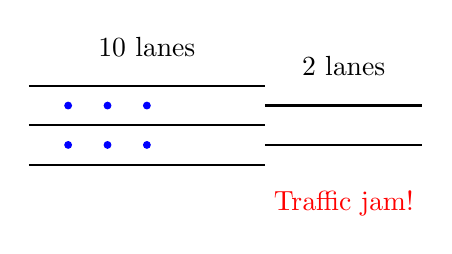
\begin{tikzpicture}[scale=1]
% Highway to city
\draw[thick] (-4,0) -- (-1,0);
\draw[thick] (-4,0.5) -- (-1,0.5);
\draw[thick] (-4,1) -- (-1,1);
\node at (-2.5,1.5) {10 lanes};

% Bottleneck
\draw[thick] (-1,0.25) -- (1,0.25);
\draw[thick] (-1,0.75) -- (1,0.75);
\node at (0,1.25) {2 lanes};
\node at (0,-0.5) {\textcolor{red}{Traffic jam!}};

% Cars
\foreach \x in {-3.5,-3,-2.5}
    \foreach \y in {0.25,0.75}
        \fill[blue] (\x,\y) circle (0.05);
\end{tikzpicture}
\end{center}

\textbf{Solution needed:} Different distance function in 2D

\note{
[1.5 min] Intuitive analogy for crowding.
}
\end{frame}

% SLIDE 29: GAUSSIAN VS T
\begin{frame}
\frametitle{The Solution: Heavy Tails}

\begin{center}
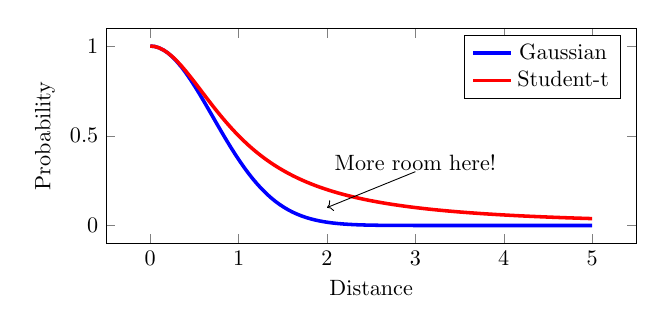
\begin{tikzpicture}[scale=0.8]
\begin{axis}[
    xlabel={Distance},
    ylabel={Probability},
    width=10cm,
    height=5cm,
    legend pos=north east,
    domain=0:5
]
\addplot[blue, ultra thick, samples=100] {exp(-x^2)};
\addlegendentry{Gaussian}

\addplot[red, ultra thick, samples=100] {1/(1+x^2)};
\addlegendentry{Student-t}

\draw[<-] (axis cs: 2,0.1) -- (axis cs: 3,0.3);
\node at (axis cs: 3,0.35) {More room here!};
\end{axis}
\end{tikzpicture}
\end{center}

Heavy tails = more probability at moderate distances

\note{
[2 min] The key insight! Visual proof.
}
\end{frame}

% SLIDE 30: T-DISTRIBUTION CHOICE
\begin{frame}
\frametitle{Why Student-t with df=1?}

\begin{columns}
\column{0.5\textwidth}
\textbf{The Choice:}
$q_{ij} \propto (1 + ||y_i - y_j||^2)^{-1}$

\vspace{0.3cm}
\textbf{Why df=1?}
\begin{itemize}
\item Heaviest tails
\item Simple gradient
\item Fast computation
\item Works best!
\end{itemize}

\column{0.5\textwidth}
\textbf{Tail Comparison:}\\
\small
\begin{tabular}{l|l}
Distribution & Decay\\
\hline
Gaussian & $e^{-d^2}$\\
t(df=1) & $d^{-2}$\\
t(df=5) & $d^{-6}$\\
\end{tabular}

\vspace{0.3cm}
df=1 gives most room!
\end{columns}

\note{
[2 min] Justify specific choice. End of first 30 slides.
}
\end{frame}

% SLIDE 31: STUDENT-T MATHEMATICAL
\begin{frame}
\frametitle{Student-t Distribution: The Mathematics}

\begin{definition}[Student-t with 1 degree of freedom]
In low dimensions, we use:
$q_{ij} = \frac{(1 + ||y_i - y_j||^2)^{-1}}{\sum_{k \neq l} (1 + ||y_k - y_l||^2)^{-1}}$
\end{definition}

\textbf{This is the Cauchy distribution:}
$f(x) = \frac{1}{\pi(1 + x^2)}$

\textbf{Key property:} Polynomial decay vs exponential

\note{
[2 min] Mathematical foundation. Note this is NOT arbitrary.
}
\end{frame}

% SLIDE 32: TAIL BEHAVIOR COMPARISON
\begin{frame}
\frametitle{Tail Behavior Analysis}

\begin{center}
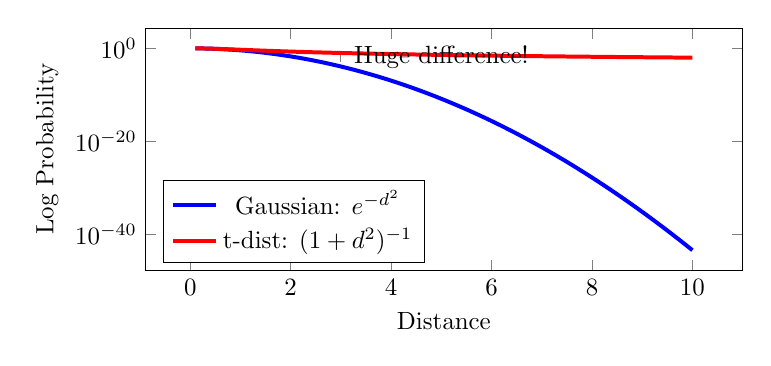
\begin{tikzpicture}[scale=0.9]
\begin{axis}[
    xlabel={Distance},
    ylabel={Log Probability},
    ymode=log,
    width=10cm,
    height=5cm,
    legend pos=south west,
    domain=0.1:10
]
\addplot[blue, ultra thick, samples=100] {exp(-x^2)};
\addlegendentry{Gaussian: $e^{-d^2}$}

\addplot[red, ultra thick, samples=100] {1/(1+x^2)};
\addlegendentry{t-dist: $(1+d^2)^{-1}$};

\draw[dashed, gray] (axis cs: 3,0.001) -- (axis cs: 3,1);
\node at (axis cs: 5,0.01) {Huge difference!};
\end{axis}
\end{tikzpicture}
\end{center}

At $d=3$: Gaussian $\approx 10^{-4}$, Student-t $\approx 0.1$

\note{
[1.5 min] Log scale reveals dramatic difference.
}
\end{frame}

% SLIDE 33: GRADIENT SIMPLIFICATION
\begin{frame}
\frametitle{The Elegant Gradient}

\begin{theorem}[t-SNE Gradient]
With Student-t in low dimensions:
$\frac{\partial C}{\partial y_i} = 4\sum_j (p_{ij} - q_{ij})(y_i - y_j)(1 + ||y_i - y_j||^2)^{-1}$
\end{theorem}

\textbf{Compare complexity:}

\begin{columns}
\column{0.5\textwidth}
\textbf{Gaussian:}
\begin{itemize}
\item Compute $e^{-||y_i - y_j||^2}$
\item Expensive exp()
\item Numerical issues
\end{itemize}

\column{0.5\textwidth}
\textbf{Student-t:}
\begin{itemize}
\item Compute $(1 + ||y_i - y_j||^2)^{-1}$
\item Simple division
\item Stable
\end{itemize}
\end{columns}

\note{
[2 min] Computational bonus - faster AND better!
}
\end{frame}

% SLIDE 34: FORCE INTERPRETATION
\begin{frame}
\frametitle{Forces in t-SNE}

\begin{center}
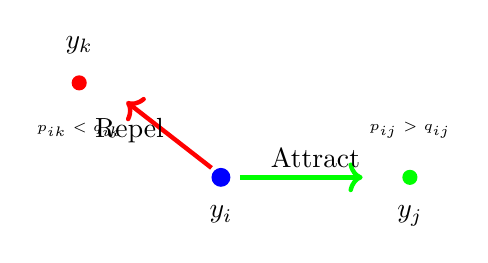
\begin{tikzpicture}[scale=1.2]
\fill[blue] (0,0) circle (0.1);
\node[below] at (0,-0.2) {$y_i$};

% Attractive force
\fill[green] (2,0) circle (0.08);
\node[below] at (2,-0.2) {$y_j$};
\draw[->, ultra thick, green] (0.2,0) -- (1.5,0);
\node[above] at (1,0) {Attract};
\node at (2,0.5) {\tiny $p_{ij} > q_{ij}$};

% Repulsive force
\fill[red] (-1.5,1) circle (0.08);
\node[above] at (-1.5,1.2) {$y_k$};
\draw[->, ultra thick, red] (-0.1,0.1) -- (-1,0.8);
\node[left] at (-0.5,0.5) {Repel};
\node at (-1.5,0.5) {\tiny $p_{ik} < q_{ik}$};
\end{tikzpicture}
\end{center}

\textbf{Spring analogy:} $(p_{ij} - q_{ij})$ = spring tension

\note{
[1.5 min] Physical interpretation helps intuition.
}
\end{frame}

% SLIDE 35: CROWDING SOLUTION VISUAL
\begin{frame}
\frametitle{How t-Distribution Solves Crowding}

\begin{center}
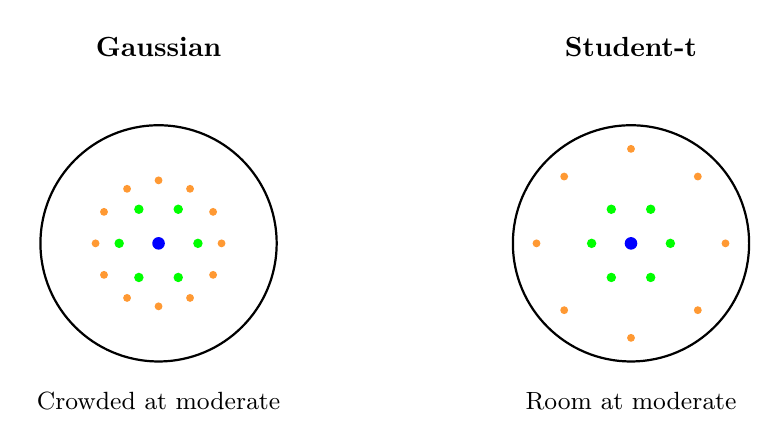
\begin{tikzpicture}[scale=1]
% Gaussian case
\node at (-3,2.5) {\textbf{Gaussian}};
\draw[thick] (-3,0) circle (1.5);
\fill[blue] (-3,0) circle (0.08);
% Close neighbors
\foreach \a in {0,60,...,300}
    \fill[green] ({-3+0.5*cos(\a)},{0.5*sin(\a)}) circle (0.06);
% Moderate - CROWDED
\foreach \a in {0,30,...,330}
    \fill[orange!80] ({-3+0.8*cos(\a)},{0.8*sin(\a)}) circle (0.05);
\node at (-3,-2) {\small Crowded at moderate};

% t-distribution case
\node at (3,2.5) {\textbf{Student-t}};
\draw[thick] (3,0) circle (1.5);
\fill[blue] (3,0) circle (0.08);
% Close neighbors
\foreach \a in {0,60,...,300}
    \fill[green] ({3+0.5*cos(\a)},{0.5*sin(\a)}) circle (0.06);
% Moderate - SPREAD OUT
\foreach \a in {0,45,...,315}
    \fill[orange!80] ({3+1.2*cos(\a)},{1.2*sin(\a)}) circle (0.05);
\node at (3,-2) {\small Room at moderate};
\end{tikzpicture}
\end{center}

\note{
[2 min] Visual proof of crowding solution.
}
\end{frame}

% SLIDE 36: PART 4 - OPTIMIZATION
\begin{frame}
\frametitle{Part 4: The Optimization Landscape}

\begin{center}
\LARGE{\textbf{Making t-SNE Work}}\\[1cm]

Key Components:
\begin{enumerate}
\item KL Divergence objective
\item Gradient descent
\item Momentum
\item Early exaggeration
\item Learning rate annealing
\end{enumerate}
\end{center}

\note{
[1 min] Transition to optimization details.
}
\end{frame}

% SLIDE 37: The Cost of a Bad Map (KL Divergence Intuition)
\begin{frame}
\frametitle{The Objective: The "Cost of a Bad Map"}

The goal is to make the low-D map ($Q$) reflect the high-D reality ($P$). The KL Divergence measures the "cost" or "penalty" for every point where the map is wrong.

\begin{center}
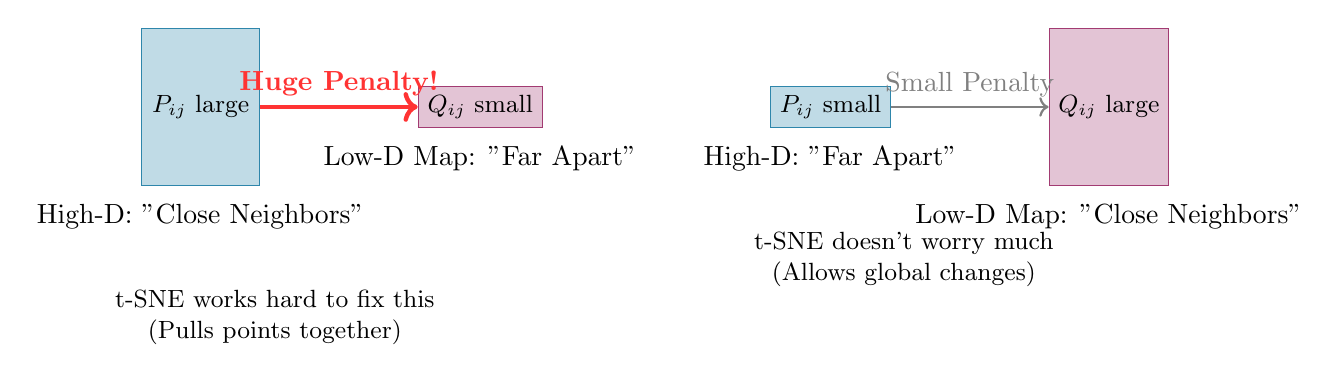
\begin{tikzpicture}[
    pbox/.style={rectangle, draw=highDcolor, fill=highDcolor!30, minimum width=1.5cm, minimum height=0.5cm, font=\small},
    qbox/.style={rectangle, draw=lowDcolor, fill=lowDcolor!30, minimum width=1.5cm, minimum height=0.5cm, font=\small},
    desc/.style={align=center, font=\small}
]
% --- Scenario 1: High Penalty ---
\begin{scope}[shift={(-4,0)}]
    \node[pbox, minimum height=2cm] (p1) {$P_{ij}$ large};
    \node[below=0.1cm of p1] {High-D: "Close Neighbors"};

    \node[qbox, minimum height=0.5cm, right=2cm of p1] (q1) {$Q_{ij}$ small};
    \node[below=0.1cm of q1] {Low-D Map: "Far Apart"};
    
    \draw[->, ultra thick, red!80] (p1.east) -- (q1.west)
        node[midway, above, font=\bfseries] {Huge Penalty!};
    \node[desc, below=1.2cm of p1.south west, xshift=1.7cm]
        {t-SNE works hard to fix this \\ (Pulls points together)};
\end{scope}

% --- Scenario 2: Low Penalty ---
\begin{scope}[shift={(4,0)}]
    \node[pbox, minimum height=0.5cm] (p2) {$P_{ij}$ small};
    \node[below=0.1cm of p2] {High-D: "Far Apart"};

    \node[qbox, minimum height=2cm, right=2cm of p2] (q2) {$Q_{ij}$ large};
    \node[below=0.1cm of q2] {Low-D Map: "Close Neighbors"};

    \draw[->, thick, gray] (p2.east) -- (q2.west)
        node[midway, above] {Small Penalty};
    \node[desc, below=1.2cm of p2.south west, xshift=1.7cm]
        {t-SNE doesn't worry much \\ (Allows global changes)};
\end{scope}
\end{tikzpicture}
\end{center}

\insight{KL Divergence cares much more about keeping close points together than pushing distant points apart.}

\note{
[2 min] This is the core intuition. Use the map analogy. A big error on your map for a short journey (Scenario 1) is a disaster. A small error for a long-distance trip you'll never take (Scenario 2) doesn't matter.
}
\end{frame}

% SLIDE 38: ASYMMETRY CONSEQUENCES
\begin{frame}
\frametitle{Asymmetry in KL Divergence}

\begin{center}
\begin{tabular}{c|c|c}
\textbf{Situation} & \textbf{Penalty} & \textbf{Effect}\\
\hline
Large $p_{ij}$, small $q_{ij}$ & \textcolor{red}{HIGH} & Preserves local\\
Small $p_{ij}$, large $q_{ij}$ & \textcolor{blue}{low} & Allows global flex\\
\end{tabular}
\end{center}

\vspace{0.5cm}
\textbf{Visual consequence:}

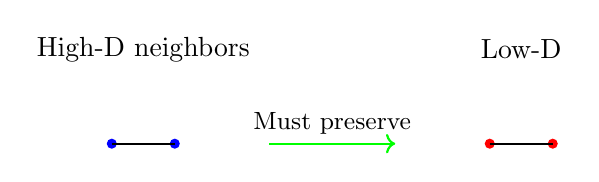
\begin{tikzpicture}[scale=0.8]
% High-D neighbors
\node at (-3,1.5) {High-D neighbors};
\fill[blue] (-3.5,0) circle (0.08);
\fill[blue] (-2.5,0) circle (0.08);
\draw[thick] (-3.5,0) -- (-2.5,0);

% Must stay together
\draw[->, thick, green] (-1,0) -- (1,0);
\node[above] at (0,0) {\small Must preserve};

% Low-D
\node at (3,1.5) {Low-D};
\fill[red] (2.5,0) circle (0.08);
\fill[red] (3.5,0) circle (0.08);
\draw[thick] (2.5,0) -- (3.5,0);
\end{tikzpicture}

\note{
  [2 min] Critical for understanding t-SNE behavior.
}
\end{frame}

% SLIDE 39: GRADIENT COMPUTATION
\begin{frame}
\frametitle{Computing the Gradient}

Starting from:
  $C = \sum_{ij} p_{ij} \log \frac{p_{ij}}{q_{ij}}$
  
  Taking derivative w.r.t. $y_i$:
  $\frac{\partial C}{\partial y_i} = 4\sum_j (p_{ij} - q_{ij})\cdot F_{ij}$
  
  where:
  $F_{ij} = \frac{(y_i - y_j)}{1 + ||y_i - y_j||^2}$
  
  \textbf{Interpretation:} Weighted sum of forces from all points

\note{
  [2 min] Mathematical derivation - show its principled.
}
\end{frame}

% SLIDE 40: EARLY EXAGGERATION
\begin{frame}
\frametitle{Early Exaggeration Trick}

\begin{columns}
\column{0.5\textwidth}
\textbf{Method:}
\begin{itemize}
\item Multiply all $p_{ij}$ by 4
\item For first 50 iterations
\item Creates tight clusters
\item Separates clusters early
\end{itemize}

\column{0.5\textwidth}
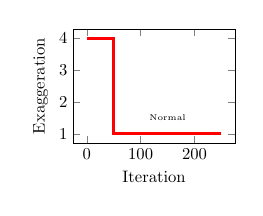
\begin{tikzpicture}[scale=0.6]
\begin{axis}[
  xlabel={Iteration},
  ylabel={Exaggeration},
  width=5cm,
  height=4cm
]
\addplot[red, ultra thick] coordinates {
  (0,4) (50,4) (50,1) (250,1)
};
\node at (axis cs: 25,4.5) {\tiny $4\times$};
\node at (axis cs: 150,1.5) {\tiny Normal};
\end{axis}
\end{tikzpicture}
\end{columns}

\vspace{0.3cm}
\textbf{Why it works:} Forces cluster formation before fine-tuning

\note{
  [1.5 min] Practical trick with big impact.
}
\end{frame}

% SLIDE 41: OPTIMIZATION ALGORITHM
\begin{frame}
\frametitle{The Complete Algorithm}

\begin{algorithmic}[1]
\State \textbf{Input:} $X \in \mathbb{R}^{n \times d}$, perplexity
\State \textbf{Output:} $Y \in \mathbb{R}^{n \times 2}$
  \State
\State Compute all $p_{ij}$ from $X$
  \State Initialize $Y \sim \mathcal{N}(0, 10^{-4}I)$
  \State
\For{iteration $t = 1$ to $T$}
\State Compute all $q_{ij}$ from $Y$
  \State Compute gradients $\frac{\partial C}{\partial Y}$
  \State Update with momentum:
  \State \quad $Y^{(t)} = Y^{(t-1)} - \eta \frac{\partial C}{\partial Y} + \alpha \Delta Y^{(t-1)}$
  \EndFor
\end{algorithmic}

\note{
  [2 min] Complete algorithm overview.
}
\end{frame}

% SLIDE 42: MOMENTUM
\begin{frame}
\frametitle{Momentum: Faster Convergence}

\begin{columns}
\column{0.5\textwidth}
\textbf{Update rule:}
$Y^{(t)} = Y^{(t-1)} - \eta \nabla + \alpha \Delta Y^{(t-1)}$
  
  where:
  \begin{itemize}
\item $\eta$: learning rate
\item $\alpha$: momentum (0.5→0.8)
\item $\Delta Y$: previous update
\end{itemize}

\column{0.5\textwidth}
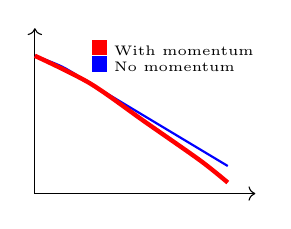
\begin{tikzpicture}[scale=0.7]
% Trajectory comparison
\draw[->] (0,0) -- (4,0);
\draw[->] (0,0) -- (0,3);
% Without momentum
\draw[blue, thick] plot[smooth] coordinates {
  (0,2.5) (0.5,2.3) (1,2.0) (1.5,1.7) (2,1.4) (2.5,1.1) (3,0.8) (3.5,0.5)
};
% With momentum
\draw[red, ultra thick] plot[smooth] coordinates {
  (0,2.5) (1,2) (2,1.3) (3,0.6) (3.5,0.2)
};
% Corrected Legend
\node[align=left, font=\tiny] at (2.5, 2.5) {
  \textcolor{red}{\rule{0.2cm}{0.2cm}} With momentum\\
  \textcolor{blue}{\rule{0.2cm}{0.2cm}} No momentum
};
\end{tikzpicture}
\end{columns}

\note{
  [1.5 min] Momentum helps escape local minima.
}
\end{frame}

% SLIDE 43: BARNES-HUT APPROXIMATION
\begin{frame}
\frametitle{Barnes-Hut: From $O(n^2)$ to $O(n\log n)$}

\begin{columns}
\column{0.5\textwidth}
\textbf{Idea:} Group distant points

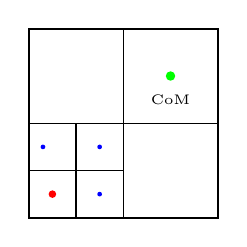
\begin{tikzpicture}[scale=0.6]
% Quadtree
\draw[thick] (0,0) rectangle (4,4);
\draw (2,0) -- (2,4);
\draw (0,2) -- (4,2);
\draw (1,0) -- (1,2);
\draw (0,1) -- (2,1);
% Points
\fill[red] (0.5,0.5) circle (0.08);
\fill[blue] (0.3,1.5) circle (0.05);
\fill[blue] (1.5,0.5) circle (0.05);
\fill[blue] (1.5,1.5) circle (0.05);
% Center of mass
\fill[green] (3,3) circle (0.1);
\node at (3,2.5) {\tiny CoM};
\end{tikzpicture}

\column{0.5\textwidth}
\textbf{Approximation:}
\begin{itemize}
\item Build quadtree
\item Compute centers of mass
\item If cell far: treat as one point
\item Threshold: $\theta = 0.5$
  \end{itemize}

\vspace{0.3cm}
\textbf{Speedup:} 100× for $n=10,000$
  \end{columns}

\note{
  [2 min] Critical for large datasets.
}
\end{frame}

% SLIDE 44: LEARNING RATE SCHEDULE
\begin{frame}
\frametitle{Learning Rate Strategies}

\begin{center}
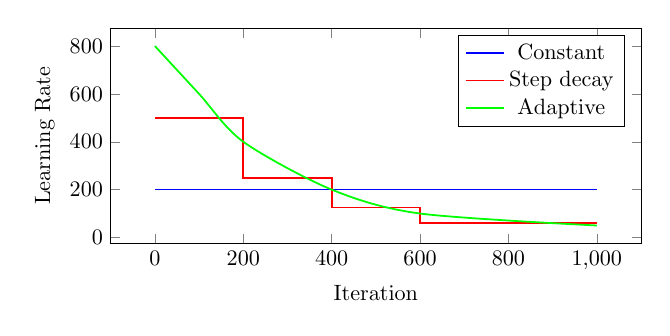
\begin{tikzpicture}[scale=0.8]
\begin{axis}[
  xlabel={Iteration},
  ylabel={Learning Rate},
  width=10cm,
  height=5cm,
  legend pos=north east
]
% Constant
\addplot[blue, thick] coordinates {
  (0,200) (1000,200)
};
\addlegendentry{Constant}

% Step decay
\addplot[red, thick] coordinates {
  (0,500) (200,500) (200,250) (400,250) (400,125) (600,125) (600,62) (1000,62)
};
\addlegendentry{Step decay}

% Adaptive
\addplot[green, thick, smooth] coordinates {
  (0,800) (100,600) (200,400) (400,200) (600,100) (1000,50)
};
\addlegendentry{Adaptive}
\end{axis}
\end{tikzpicture}
\end{center}

\textbf{Recommendation:} Start high (500-1000), decrease if needed

\note{
  [1.5 min] Learning rate crucial for convergence.
}
\end{frame}

% SLIDE 45: INITIALIZATION STRATEGIES
\begin{frame}
\frametitle{Smart Initialization}

\begin{center}
\begin{tabular}{l|l|l}
\textbf{Method} & \textbf{Pros} & \textbf{Cons}\\
\hline
Random small & No bias & Slow start\\
PCA & Fast convergence & May bias\\
Previous run & Reproducible & Local minimum\\
\end{tabular}
\end{center}

\vspace{0.5cm}
\textbf{Best practice:}
$Y_i \sim \mathcal{N}(0, 10^{-4}I)$
  
  Small variance prevents early numerical issues

\note{
  [1.5 min] Initialization affects convergence.
}
\end{frame}

% SLIDE 46: HYPERPARAMETER GRID
\begin{frame}
\frametitle{Hyperparameter Impact}

\begin{center}
\small
\begin{tabular}{l|c|c|c}
\textbf{Parameter} & \textbf{Low} & \textbf{Default} & \textbf{High}\\
\hline
Perplexity & 5-15 & 30 & 50-100\\
Learning rate & 10-100 & 200 & 500-1000\\
Iterations & 250 & 1000 & 5000\\
Momentum & 0.5 & 0.8 & 0.9\\
Early exag. & 4 & 12 & 20\\
\end{tabular}
\end{center}

\vspace{0.3cm}
\textbf{Grid search often needed for optimal results}

\note{
  [2 min] Practical guidance for users.
}
\end{frame}

% SLIDE 47: PERPLEXITY EFFECTS DETAILED
\begin{frame}
\frametitle{Perplexity: Detailed Effects}

\begin{center}
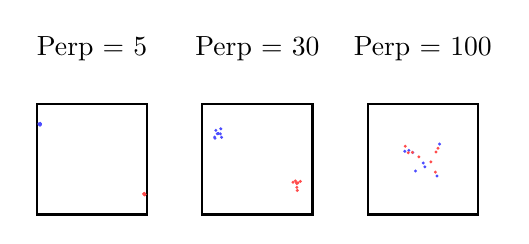
\begin{tikzpicture}[scale=0.7]
% Create 3x3 grid showing different perplexities
% CORRECTED: Renamed loop variable from \perp to \myperp
\foreach \myperp/\x in {5/-3,30/0,100/3} {
  \node at (\x,2) {Perp = \myperp};
  \draw[thick] (\x-1,-1) rectangle (\x+1,1);
  
  % Draw clusters based on perplexity
  \pgfmathsetmacro{\spread}{0.1*\myperp/30}
  \pgfmathsetmacro{\sep}{2-\myperp/50}
  
  \foreach \i in {1,...,8} {
    \pgfmathsetmacro{\rx}{rand*\spread}
    \pgfmathsetmacro{\ry}{rand*\spread}
    \fill[blue!70] ({\x+\rx-\sep/2},{\ry+\sep/3}) circle (0.03);
  }
  \foreach \i in {1,...,8} {
    \pgfmathsetmacro{\rx}{rand*\spread}
    \pgfmathsetmacro{\ry}{rand*\spread}
    \fill[red!70] ({\x+\rx+\sep/2},{\ry-\sep/3}) circle (0.03);
  }
}
\end{tikzpicture}
\end{center}

\begin{itemize}
\item \textbf{Too low:} Breaks clusters into fragments
\item \textbf{Too high:} Merges distinct clusters
\item \textbf{Sweet spot:} Usually 5-50, dataset dependent
\end{itemize}

\note{
  [2 min] Visual guide for perplexity selection.
}
\end{frame}


% SLIDE 48: LEARNING RATE SENSITIVITY
\begin{frame}
\frametitle{Learning Rate: Finding Balance}

\begin{columns}
\column{0.5\textwidth}
\textbf{Too low ($\eta < 10$):}
\begin{itemize}
\item Stuck in bad minimum
\item Slow convergence
\item Poor separation
\end{itemize}

\textbf{Too high ($\eta > 1000$):}
\begin{itemize}
\item Points explode
\item Oscillations
\item Never converges
\end{itemize}

\column{0.5\textwidth}
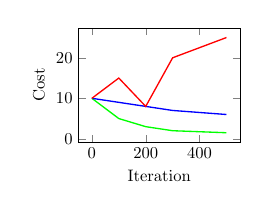
\begin{tikzpicture}[scale=0.6]
\begin{axis}[
  xlabel={Iteration},
  ylabel={Cost},
  width=5cm,
  height=4cm
]
% Good
\addplot[green, thick] coordinates {
  (0,10) (100,5) (200,3) (300,2) (500,1.5)
};
% Too low
\addplot[blue, thick] coordinates {
  (0,10) (100,9) (200,8) (300,7) (500,6)
};
% Too high
\addplot[red, thick] coordinates {
  (0,10) (100,15) (200,8) (300,20) (500,25)
};
\end{axis}
\end{tikzpicture}
\end{columns}

\note{
  [1.5 min] Critical parameter for convergence.
}
\end{frame}

% SLIDE 49: CONVERGENCE MONITORING
\begin{frame}
\frametitle{Monitoring Convergence}

\begin{columns}
\column{0.5\textwidth}
\textbf{Watch for:}
\begin{itemize}
\item KL divergence decrease
\item Gradient norm → 0
\item Stable embedding
\end{itemize}

\textbf{Warning signs:}
\begin{itemize}
\item Increasing cost
\item Points at infinity
\item Oscillations
\end{itemize}

\column{0.5\textwidth}
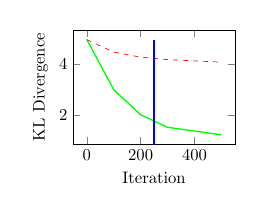
\begin{tikzpicture}[scale=0.6]
\begin{axis}[
  xlabel={Iteration},
  ylabel={KL Divergence},
  width=5cm,
  height=4cm
]
\addplot[green, thick] coordinates {
  (0,5) (100,3) (200,2) (300,1.5) (500,1.2)
};
\addplot[red, dashed] coordinates {
  (0,5) (100,4.5) (200,4.3) (300,4.2) (500,4.1)
};
\draw[blue, thick] (axis cs: 250,0) -- (axis cs: 250,5);
\node at (axis cs: 250,0.5) {\tiny Stop?};
\end{axis}
\end{tikzpicture}
\end{columns}

\note{
  [1.5 min] How to know when to stop.
}
\end{frame}

% SLIDE 50: PARAMETER EXPLORATION
\begin{frame}
\frametitle{Interactive Parameter Exploration}

\begin{center}
\textbf{Recommended workflow:}
\end{center}

\begin{enumerate}
\item Start with defaults (perp=30, lr=200)
\item Run 5 times with different seeds
\item If inconsistent: adjust perplexity
\item If slow: increase learning rate
\item If unstable: decrease learning rate
\item Compare multiple perplexity values
\end{enumerate}

\vspace{0.3cm}
\colorbox{yellow!20}{Always run multiple times - t-SNE is stochastic!}

\note{
  [2 min] Practical workflow for users.
}
\end{frame}

% SLIDE 51: PART 5 - INTERPRETATION
\begin{frame}
\frametitle{Part 5: Interpretation \& Best Practices}

\begin{center}
\LARGE{\textbf{Reading t-SNE Correctly}}\\[1cm]

Critical questions:
  \begin{itemize}
\item What can we trust?
  \item What is meaningless?
  \item How to validate?
  \end{itemize}
\end{center}

\note{
  [1 min] Transition to interpretation.
}
\end{frame}

% SLIDE 52: WHAT TO TRUST
\begin{frame}
\frametitle{What You Can Trust}

\begin{columns}
\column{0.5\textwidth}
\textbf{\textcolor{green}{Can Trust:}}
\begin{itemize}
\item Local neighborhoods
\item Cluster existence
\item Within-cluster structure
\item Relative densities (roughly)
\end{itemize}

\column{0.5\textwidth}
\textbf{\textcolor{red}{Cannot Trust:}}
\begin{itemize}
\item Cluster sizes
\item Between-cluster distances
\item Global structure
\item Absolute positions
\end{itemize}
\end{columns}

\vspace{0.5cm}
\centering
\colorbox{red!20}{t-SNE is for exploration, not measurement!}

\note{
  [2 min] Critical distinctions for interpretation.
}
\end{frame}

% SLIDE 53: CLUSTER SEPARATION
\begin{frame}
\frametitle{Cluster Separation: Real or Artifact?}

\begin{center}
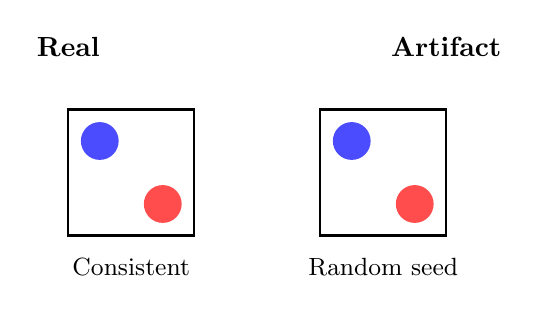
\begin{tikzpicture}[scale=0.8]
% Real separation
\node at (-3,2) {\textbf{Real}};
\draw[thick] (-3,-1) rectangle (-1,1);
\fill[blue!70] (-2.5,0.5) circle (0.3);
\fill[red!70] (-1.5,-0.5) circle (0.3);
\node at (-2,-1.5) {\small Consistent};

% Artifact
\node at (3,2) {\textbf{Artifact}};
\draw[thick] (1,-1) rectangle (3,1);
\fill[blue!70] (1.5,0.5) circle (0.3);
\fill[red!70] (2.5,-0.5) circle (0.3);
\node at (2,-1.5) {\small Random seed};
\end{tikzpicture}
\end{center}

\textbf{Validation:} Run multiple times, check if stable

\note{
  [1.5 min] How to distinguish real from artifacts.
}
\end{frame}

% SLIDE 54: DISTANCE INTERPRETATION
\begin{frame}
\frametitle{Distance Interpretation Warnings}

\begin{center}
\textbf{Between-cluster distances are meaningless!}

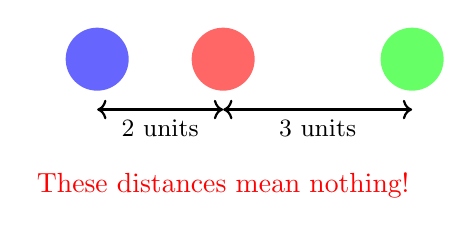
\begin{tikzpicture}[scale=0.8]
\fill[blue!60] (-2,0) circle (0.5);
\fill[red!60] (0,0) circle (0.5);
\fill[green!60] (3,0) circle (0.5);

\draw[<->, thick] (-2,-0.8) -- (0,-0.8);
\node at (-1,-1.1) {\small 2 units};

\draw[<->, thick] (0,-0.8) -- (3,-0.8);
\node at (1.5,-1.1) {\small 3 units};

\node at (0,-2) {\textcolor{red}{These distances mean nothing!}};
\end{tikzpicture}
\end{center}

In high-D, all three might be equidistant

\note{
  [1.5 min] Common misinterpretation to avoid.
}
\end{frame}

% SLIDE 55: CLUSTER SIZE
\begin{frame}
\frametitle{Cluster Size Non-Preservation}

\begin{columns}
\column{0.5\textwidth}
\textbf{High-D Reality:}
\begin{itemize}
\item Cluster A: 1000 points
\item Cluster B: 100 points
\item Ratio: 10:1
\end{itemize}

\column{0.5\textwidth}
\textbf{t-SNE Display:}
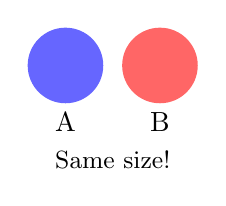
\begin{tikzpicture}[scale=0.6]
\fill[blue!60] (0,0) circle (0.8);
\fill[red!60] (2,0) circle (0.8);
\node at (0,-1.2) {A};
\node at (2,-1.2) {B};
\node at (1,-2) {\small Same size!};
\end{tikzpicture}
\end{columns}

\vspace{0.5cm}
\textbf{Why:} Optimization doesnt preserve density

\note{
[1.5 min] Important limitation to communicate.
}
\end{frame}

% SLIDE 56: COMMON PITFALL - LOW PERPLEXITY
\begin{frame}
\frametitle{Pitfall: Perplexity Too Low}

\begin{center}
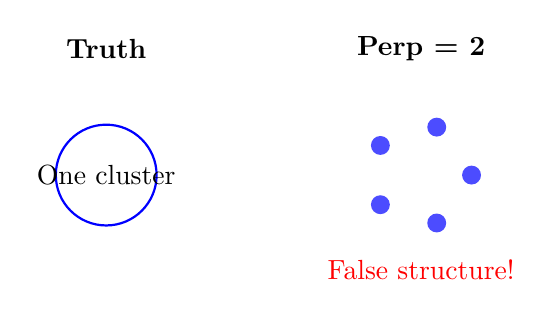
\begin{tikzpicture}[scale=0.8]
% Original
\node at (-3,2) {\textbf{Truth}};
\draw[thick, blue] (-3,0) circle (0.8);
\node at (-3,0) {One cluster};

% After t-SNE with low perp
\node at (2,2) {\textbf{Perp = 2}};
\foreach \a in {0,72,...,288} {
    \fill[blue!70] ({2+0.8*cos(\a)},{0.8*sin(\a)}) circle (0.15);
}
\node at (2,-1.5) {\textcolor{red}{False structure!}};
\end{tikzpicture}
\end{center}

\textbf{Solution:} Increase perplexity to 15+

\note{
[1.5 min] Very common mistake.
}
\end{frame}

% SLIDE 57: PITFALL - HIGH PERPLEXITY
\begin{frame}
\frametitle{Pitfall: Perplexity Too High}

\begin{center}
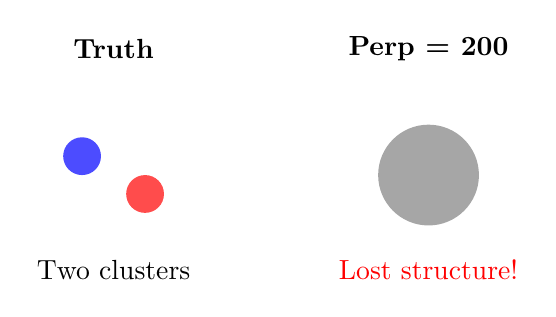
\begin{tikzpicture}[scale=0.8]
% Original
\node at (-3,2) {\textbf{Truth}};
\fill[blue!70] (-3.5,0.3) circle (0.3);
\fill[red!70] (-2.5,-0.3) circle (0.3);
\node at (-3,-1.5) {Two clusters};

% After t-SNE with high perp
\node at (2,2) {\textbf{Perp = 200}};
\fill[gray!70] (2,0) circle (0.8);
\node at (2,-1.5) {\textcolor{red}{Lost structure!}};
\end{tikzpicture}
\end{center}

\textbf{Solution:} Decrease perplexity to 30-50

\note{
[1.5 min] Opposite problem.
}
\end{frame}

% SLIDE 58: NON-CONVERGENCE
\begin{frame}
\frametitle{Pitfall: Non-Convergence}

\begin{columns}
\column{0.5\textwidth}
\textbf{Symptoms:}
\begin{itemize}
\item Points still moving
\item Cost oscillating
\item Clusters not separated
\end{itemize}

\textbf{Solutions:}
\begin{itemize}
\item More iterations (2000+)
\item Adjust learning rate
\item Check for outliers
\end{itemize}

\column{0.5\textwidth}
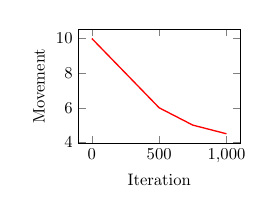
\begin{tikzpicture}[scale=0.6]
\begin{axis}[
    xlabel={Iteration},
    ylabel={Movement},
    width=5cm,
    height=4cm
]
\addplot[red, thick] coordinates {
    (0,10) (250,8) (500,6) (750,5) (1000,4.5)
};
\draw[dashed] (axis cs: 0,0.1) -- (axis cs: 1000,0.1);
\node at (axis cs: 500,1) {\tiny Not converged};
\end{axis}
\end{tikzpicture}
\end{columns}

\note{
[1.5 min] How to diagnose convergence issues.
}
\end{frame}

% SLIDE 59: OUTLIER EFFECTS
\begin{frame}
\frametitle{Outlier Effects}

\begin{center}
\begin{tikzpicture}[scale=0.8]
% Normal data
\foreach \i in {1,...,20} {
    \pgfmathsetmacro{\rx}{rand*2}
    \pgfmathsetmacro{\ry}{rand*2}
    \fill[blue!60] (\rx,\ry) circle (0.05);
}
% Outlier
\fill[red] (4,4) circle (0.1);
\draw[red, thick] (3.5,3.5) -- (4.5,4.5);
\node at (4.5,4.5) {\small Outlier};

% Effect arrow
\draw[->, ultra thick, red] (2.5,2.5) -- (3.5,3.5);
\node at (2,3) {Pulls structure};
\end{tikzpicture}
\end{center}

\textbf{Solutions:}
\begin{itemize}
\item Remove extreme outliers first
\item Use robust preprocessing
\item Check with and without outliers
\end{itemize}

\note{
[1.5 min] Outliers can distort entire embedding.
}
\end{frame}

% SLIDE 60: REPRODUCIBILITY
\begin{frame}
\frametitle{Ensuring Reproducibility}

\begin{enumerate}
\item \textbf{Set random seed}
\begin{itemize}
\item For initialization
\item For algorithm
\end{itemize}

\item \textbf{Document parameters}
\begin{itemize}
\item Perplexity
\item Learning rate
\item Iterations
\end{itemize}

\item \textbf{Save intermediate states}
\begin{itemize}
\item Every 100 iterations
\item For debugging
\end{itemize}
\end{enumerate}

\colorbox{green!20}{Always report: "t-SNE with perp=X, lr=Y, iter=Z"}

\note{
[1.5 min] Scientific reproducibility essential.
}
\end{frame}

% SLIDE 61: ADVANCED - PARAMETRIC t-SNE
\begin{frame}
\frametitle{Advanced: Parametric t-SNE}

\begin{columns}
\column{0.5\textwidth}
\textbf{Idea:} Learn a function $f: \mathbb{R}^d \rightarrow \mathbb{R}^2$

\textbf{Advantages:}
\begin{itemize}
\item Can embed new points
\item Inverse mapping possible
\item Interpretable features
\end{itemize}

\column{0.5\textwidth}
\textbf{Neural Network:}
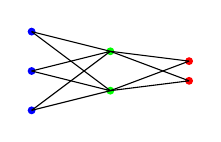
\begin{tikzpicture}[scale=0.5]
% Input layer
\foreach \y in {0,1,2}
    \fill[blue] (0,\y) circle (0.1);
% Hidden layer
\foreach \y in {0.5,1.5}
    \fill[green] (2,\y) circle (0.1);
% Output layer
\foreach \y in {0.75,1.25}
    \fill[red] (4,\y) circle (0.1);
% Connections - fixed version
\foreach \ya in {0,1,2} {
    \foreach \yb in {0.5,1.5} {
        \draw (0,\ya) -- (2,\yb);
    }
}
\foreach \ya in {0.5,1.5} {
    \foreach \yb in {0.75,1.25} {
        \draw (2,\ya) -- (4,\yb);
    }
}
\end{tikzpicture}
\end{columns}

\note{
[2 min] Extension for production systems.
}
\end{frame}

% SLIDE 62: MULTI-SCALE t-SNE
\begin{frame}
\frametitle{Advanced: Multi-Scale t-SNE}

\begin{center}
\textbf{Use multiple perplexities simultaneously}

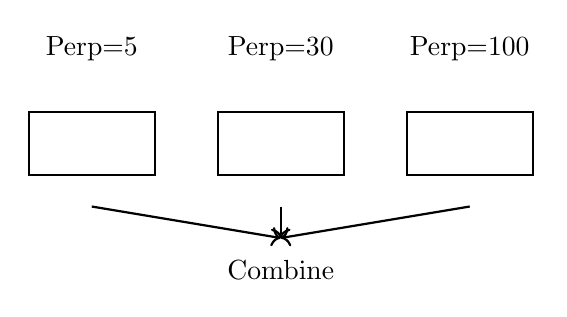
\begin{tikzpicture}[scale=0.8]
% Perp 5
\node at (-3,2) {Perp=5};
\draw[thick] (-4,0) rectangle (-2,1);
% Perp 30
\node at (0,2) {Perp=30};
\draw[thick] (-1,0) rectangle (1,1);
% Perp 100
\node at (3,2) {Perp=100};
\draw[thick] (2,0) rectangle (4,1);

% Combination
\draw[->, thick] (-3,-0.5) -- (0,-1);
\draw[->, thick] (0,-0.5) -- (0,-1);
\draw[->, thick] (3,-0.5) -- (0,-1);
\node at (0,-1.5) {Combine};
\end{tikzpicture}
\end{center}

$p_{ij} = \sum_{k} w_k \cdot p_{ij}^{(perp_k)}$

Captures both local and global structure

\note{
[1.5 min] Advanced technique for complex data.
}
\end{frame}

% SLIDE 63: DYNAMIC t-SNE
\begin{frame}
\frametitle{Advanced: Dynamic t-SNE}

\textbf{For temporal data:} Preserve structure over time

\begin{center}
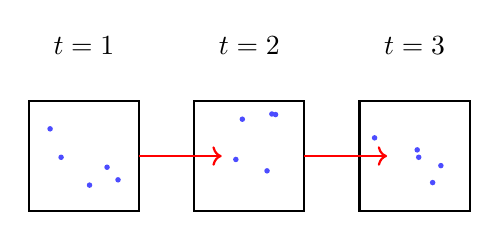
\begin{tikzpicture}[scale=0.7]
% Time steps
\foreach \t/\x in {1/-3,2/0,3/3} {
    \node at (\x,2) {$t=\t$};
    \draw[thick] (\x-1,-1) rectangle (\x+1,1);
    % Points
    \foreach \i in {1,...,5} {
        \pgfmathsetmacro{\rx}{rand*0.8}
        \pgfmathsetmacro{\ry}{rand*0.8}
        \fill[blue!70] ({\x+\rx},\ry) circle (0.05);
    }
}
% Temporal links
\draw[->, thick, red] (-2,0) -- (-0.5,0);
\draw[->, thick, red] (1,0) -- (2.5,0);
\end{tikzpicture}
\end{center}

Add temporal regularization: $\lambda||Y_t - Y_{t-1}||^2$

\note{
[1.5 min] For time series visualization.
}
\end{frame}

% SLIDE 64: t-SNE vs UMAP
\begin{frame}
\frametitle{t-SNE vs UMAP}

\begin{center}
\small
\begin{tabular}{l|c|c}
\textbf{Aspect} & \textbf{t-SNE} & \textbf{UMAP}\\
\hline
Speed & $O(n \log n)$ & $O(n^{1.14})$\\
Theory & Probability & Topology\\
Global structure & Poor & Better\\
Parameters & Perplexity & n\_neighbors\\
Reproducibility & Random & More stable\\
Scalability & <50K points & Millions\\
\end{tabular}
\end{center}

\vspace{0.3cm}
\textbf{When to use each:}
\begin{itemize}
\item t-SNE: Exploring clusters, publication figures
\item UMAP: Large data, need global structure
\end{itemize}

\note{
[2 min] Modern alternative comparison.
}
\end{frame}

% SLIDE 65: RECENT DEVELOPMENTS
\begin{frame}
\frametitle{Research Frontiers}

\begin{enumerate}
\item \textbf{Initialization:} PaCMAP, TriMAP
\item \textbf{Speed:} FIt-SNE, openTSNE
\item \textbf{Theory:} Heavy-tailed embeddings
\item \textbf{Interpretability:} Attribution methods
\item \textbf{Uncertainty:} Probabilistic embeddings
\end{enumerate}

\vspace{0.3cm}
\textbf{Active research area:} 100+ papers/year

\note{
[1.5 min] Field is still evolving.
}
\end{frame}

% SLIDE 66: PART 6 - IMPLEMENTATION
\begin{frame}
\frametitle{Part 6: Practical Implementation}

\begin{center}
\LARGE{\textbf{From Theory to Code}}\\[1cm]

Ready to implement t-SNE!
\end{center}

\note{
[1 min] Transition to practical.
}
\end{frame}

% SLIDE 67: PYTHON IMPLEMENTATION
\begin{frame}[fragile]
\frametitle{Python: scikit-learn}

\begin{verbatim}
from sklearn.manifold import TSNE
import numpy as np

# Your data: n_samples × n_features
X = load_data()

# Configure t-SNE
tsne = TSNE(n_components=2,
            perplexity=30,
            learning_rate=200,
            n_iter=1000,
            random_state=42)

# Fit and transform
Y = tsne.fit_transform(X)

# Visualize
plt.scatter(Y[:, 0], Y[:, 1])
\end{verbatim}

\note{
[2 min] Standard implementation.
}
\end{frame}

% SLIDE 68: R IMPLEMENTATION
\begin{frame}[fragile]
\frametitle{R: Rtsne Package}

\begin{verbatim}
library(Rtsne)

# Prepare data
X <- as.matrix(your_data)

# Run t-SNE
tsne_out <- Rtsne(X,
                   dims = 2,
                   perplexity = 30,
                   theta = 0.5,
                   max_iter = 1000)

# Extract embedding
Y <- tsne_out$Y

# Plot
plot(Y, col = labels)
\end{verbatim}

\note{
[2 min] R users implementation.
}
\end{frame}

% SLIDE 69: KEY PARAMETERS
\begin{frame}
\frametitle{Key Parameters Explained}

\begin{center}
\small
\begin{tabular}{l|l|l}
\textbf{Parameter} & \textbf{Meaning} & \textbf{Guidance}\\
\hline
perplexity & Neighborhood size & 5-50\\
learning\_rate & Step size & 10-1000\\
n\_iter & Iterations & 250-5000\\
theta & Barnes-Hut accuracy & 0.5 default\\
metric & Distance function & euclidean\\
init & Initialization & pca or random\\
\end{tabular}
\end{center}

\vspace{0.3cm}
\textbf{Most important:} perplexity and learning\_rate

\note{
[1.5 min] Parameter reference guide.
}
\end{frame}

% SLIDE 70: OPTIMIZATION TIPS
\begin{frame}
\frametitle{Performance Optimization}

\begin{enumerate}
\item \textbf{Preprocessing:}
\begin{itemize}
\item PCA to 50D first
\item Normalize features
\item Remove duplicates
\end{itemize}

\item \textbf{Computation:}
\begin{itemize}
\item Use float32 not float64
\item Enable multicore
\item GPU versions available
\end{itemize}

\item \textbf{Large datasets:}
\begin{itemize}
\item Sample first, then embed
\item Use UMAP for >100K points
\item Consider parametric t-SNE
\end{itemize}
\end{enumerate}

\note{
[2 min] Practical speedup tips.
}
\end{frame}

% SLIDE 71: CASE STUDY - GENOMICS
\begin{frame}
\frametitle{Case Study: Single-Cell RNA-seq}

\begin{columns}
\column{0.5\textwidth}
\textbf{Dataset:}
\begin{itemize}
\item 10,000 cells
\item 20,000 genes
\item Goal: Find cell types
\end{itemize}

\textbf{Pipeline:}
\begin{enumerate}
\item Filter genes (variance)
\item Log transform
\item PCA to 50D
\item t-SNE with perp=30
\end{enumerate}

\column{0.5\textwidth}
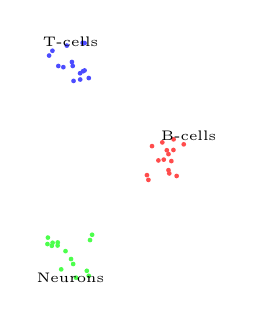
\begin{tikzpicture}[scale=0.6]
% Cell type clusters
\foreach \i in {1,...,15} {
    \pgfmathsetmacro{\rx}{rand*0.5}
    \pgfmathsetmacro{\ry}{rand*0.5}
    \fill[blue!70] (\rx,{\ry+2}) circle (0.05);
}
\foreach \i in {1,...,15} {
    \pgfmathsetmacro{\rx}{rand*0.5}
    \pgfmathsetmacro{\ry}{rand*0.5}
    \fill[red!70] ({\rx+2},\ry) circle (0.05);
}
\foreach \i in {1,...,15} {
    \pgfmathsetmacro{\rx}{rand*0.5}
    \pgfmathsetmacro{\ry}{rand*0.5}
    \fill[green!70] (\rx,{\ry-2}) circle (0.05);
}
\node at (0,2.5) {\tiny T-cells};
\node at (2.5,0.5) {\tiny B-cells};
\node at (0,-2.5) {\tiny Neurons};
\end{tikzpicture}
\end{columns}

\note{
[2 min] Real application example.
}
\end{frame}

% SLIDE 72: CASE STUDY - VISION
\begin{frame}
\frametitle{Case Study: ImageNet Features}

\begin{columns}
\column{0.5\textwidth}
\textbf{Setup:}
\begin{itemize}
\item CNN features (2048D)
\item 50,000 images
\item 1000 classes
\end{itemize}

\textbf{Results:}
\begin{itemize}
\item Similar objects cluster
\item Hierarchical structure
\item Visual similarity preserved
\end{itemize}

\column{0.5\textwidth}
\begin{tikzpicture}[scale=0.5]
% Animal cluster
\fill[brown!60] (0,2) circle (0.8);
\node at (0,2) {\tiny Animals};
% Vehicle cluster
\fill[blue!60] (3,2) circle (0.8);
\node at (3,2) {\tiny Vehicles};
% Plants cluster
\fill[green!60] (1.5,-1) circle (0.8);
\node at (1.5,-1) {\tiny Plants};
\end{tikzpicture}
\end{columns}

\note{
[1.5 min] Computer vision application.
}
\end{frame}

% SLIDE 73: CASE STUDY - NLP
\begin{frame}
\frametitle{Case Study: Word Embeddings}

\begin{center}
\textbf{Word2Vec embeddings (300D) → t-SNE (2D)}

\begin{tikzpicture}[scale=0.8]
% Countries
\fill[blue!30] (-2,2) circle (0.8);
\node at (-2,2) {\tiny Countries};
\node at (-2.2,2.2) {\tiny France};
\node at (-1.8,1.8) {\tiny Spain};

% Colors
\fill[red!30] (2,2) circle (0.8);
\node at (2,2) {\tiny Colors};
\node at (2.2,2.2) {\tiny red};
\node at (1.8,1.8) {\tiny blue};

% Actions
\fill[green!30] (0,-1) circle (0.8);
\node at (0,-1) {\tiny Actions};
\node at (0.2,-0.8) {\tiny run};
\node at (-0.2,-1.2) {\tiny walk};
\end{tikzpicture}
\end{center}

Semantic relationships preserved!

\note{
[1.5 min] NLP application showing semantic clustering.
}
\end{frame}

% SLIDE 74: CASE STUDY - TIME SERIES
\begin{frame}
\frametitle{Case Study: Financial Time Series}

\begin{columns}
\column{0.5\textwidth}
\textbf{Data:}
\begin{itemize}
\item Stock returns
\item 500 companies
\item 252 trading days
\end{itemize}

\textbf{Preprocessing:}
\begin{itemize}
\item Correlation matrix
\item t-SNE embedding
\item Color by sector
\end{itemize}

\column{0.5\textwidth}
\begin{tikzpicture}[scale=0.5]
% Tech sector
\fill[blue!60] (-1,2) circle (0.6);
\node at (-1,2) {\tiny Tech};
% Finance sector
\fill[red!60] (2,1) circle (0.6);
\node at (2,1) {\tiny Finance};
% Energy sector
\fill[green!60] (0,-1) circle (0.6);
\node at (0,-1) {\tiny Energy};
\end{tikzpicture}

Sectors naturally separate!
\end{columns}

\note{
[1.5 min] Financial application.
}
\end{frame}

% SLIDE 75: YOUR RESEARCH
\begin{frame}
\frametitle{Apply to Your Research}

\begin{center}
\textbf{t-SNE Checklist:}
\end{center}

\begin{enumerate}
\item Is your data high-dimensional? (d > 10)
\item Do you want to explore structure?
\item Is $n < 50,000$?
\item Can you validate clusters independently?
\end{enumerate}

\vspace{0.3cm}
If yes to all → t-SNE is perfect!

\vspace{0.3cm}
\textbf{Remember:}
\begin{itemize}
\item Try multiple perplexities
\item Run multiple times
\item Validate findings
\end{itemize}

\note{
[2 min] Encourage application to own work.
}
\end{frame}

% SLIDE 76: PART 7 - KEY TAKEAWAYS
\begin{frame}
\frametitle{Part 7: Synthesis}

\begin{center}
\LARGE{\textbf{Key Takeaways}}\\[1cm]

What you have mastered today
\end{center}

\note{
[1 min] Final section transition.
}
\end{frame}

% SLIDE 77: WHEN TO USE t-SNE
\begin{frame}
\frametitle{When to Use t-SNE}

\begin{columns}
\column{0.5\textwidth}
\textbf{\textcolor{green}{Use t-SNE:}}
\begin{itemize}
\item Exploring clusters
\item Validating features
\item Finding outliers
\item Publication figures
\item Quality over speed
\end{itemize}

\column{0.5\textwidth}
\textbf{\textcolor{red}{Dont use t-SNE:}}
\begin{itemize}
\item Measuring distances
\item $>$ 100K points
\item Real-time analysis
\item Definitive proof
\item Production systems
\end{itemize}
\end{columns}

\vspace{0.5cm}
\centering
\colorbox{blue!20}{t-SNE is for exploration and insight}

\note{
[2 min] Clear guidance on appropriate use.
}
\end{frame}

% SLIDE 78: INTERPRETATION CHECKLIST
\begin{frame}
\frametitle{The Interpretation Checklist}

Before publishing t-SNE results:

\begin{enumerate}
\item $\square$ Tried perplexity: 5, 15, 30, 50
\item $\square$ Ran 5+ random initializations
\item $\square$ Checked convergence (1000+ iterations)
\item $\square$ Validated clusters independently
\item $\square$ Stated all parameters clearly
\item $\square$ Acknowledged limitations
\item $\square$ Compared with PCA/other methods
\end{enumerate}

\vspace{0.3cm}
\colorbox{yellow!20}{Never interpret distances or sizes!}

\note{
[2 min] Essential checklist for rigorous use.
}
\end{frame}

% SLIDE 79: RESOURCES
\begin{frame}
\frametitle{Resources for Deeper Study}

\textbf{Essential Papers:}
\begin{itemize}
\item Original: van der Maaten \& Hinton (2008)
\item Barnes-Hut: van der Maaten (2014)
\item Theory: Linderman \& Steinerberger (2017)
\end{itemize}

\textbf{Software:}
\begin{itemize}
\item Python: scikit-learn, openTSNE
\item R: Rtsne, tsne
\item Fast: FIt-SNE, RAPIDS
\end{itemize}

\textbf{Tutorials:}
\begin{itemize}
\item Distill.pub interactive guide
\item Google embedding projector
\end{itemize}

\note{
[1.5 min] Where to learn more.
}
\end{frame}

% SLIDE 80: DISCUSSION & Q&A
\begin{frame}
\frametitle{Discussion \& Questions}

\begin{center}
\LARGE{\textbf{Your Questions?}}\\[1cm]

\begin{tikzpicture}[scale=1]
\draw[thick, rounded corners] (-2.5,-1) rectangle (2.5,1);
\node at (0,0) {
    \begin{tabular}{c}
    Theory?\\
    Implementation?\\
    Your data?
    \end{tabular}
};
\end{tikzpicture}
\end{center}

\vspace{0.5cm}
\centering
\textit{Thank you for your attention!}\\
\textit{Now lets explore your data with t-SNE!}

\note{
[10 min] Open discussion. Encourage specific questions about their research.
}
\end{frame}

\end{document}

